\documentclass[11pt]{amsart}
\usepackage[T1]{fontenc}
\usepackage{lmodern}
\usepackage{amsmath,amssymb,amscd,mathtools}
\usepackage{mathrsfs}
\usepackage[margin=1.05in]{geometry}
\usepackage{microtype}
\usepackage{needspace}
\usepackage{enumitem}
\usepackage{tikz}
\usetikzlibrary{arrows.meta,positioning,calc}
\usepackage[hidelinks,pdfauthor={OpenAI},pdftitle={Constructible tame Hecke eigensheaves in positive characteristic}]{hyperref}
\numberwithin{equation}{section}
\newtheorem{theorem}{Theorem}[section]
\newtheorem{lemma}[theorem]{Lemma}
\newtheorem{proposition}[theorem]{Proposition}
\newtheorem{corollary}[theorem]{Corollary}
\newtheorem{claim}[theorem]{Claim}
\theoremstyle{definition}
\newtheorem{definition}[theorem]{Definition}
\newtheorem{convention}[theorem]{Convention}
\newtheorem{assumption}[theorem]{Assumption}
\theoremstyle{remark}
\newtheorem{remark}[theorem]{Remark}
\newtheorem{example}[theorem]{Example}
\DeclareMathOperator{\Bun}{Bun}
\DeclareMathOperator{\Loc}{Loc}
\DeclareMathOperator{\LS}{LS}
\let\SS\relax
\DeclareMathOperator{\SS}{SS}
\DeclareMathOperator{\QCoh}{QCoh}
\DeclareMathOperator{\IndCoh}{IndCoh}
\DeclareMathOperator{\Perf}{Perf}
\DeclareMathOperator{\Rep}{Rep}
\DeclareMathOperator{\Spec}{Spec}
\DeclareMathOperator{\Lie}{Lie}
\DeclareMathOperator{\ad}{ad}
\DeclareMathOperator{\Ad}{Ad}
\DeclareMathOperator{\IC}{IC}
\DeclareMathOperator{\Gr}{Gr}
\DeclareMathOperator{\Fl}{Fl}
\DeclareMathOperator{\Shv}{Shv}
\DeclareMathOperator{\Perv}{Perv}
\DeclareMathOperator{\Hom}{Hom}
\DeclareMathOperator{\End}{End}
\DeclareMathOperator{\Aut}{Aut}
\DeclareMathOperator{\im}{im}
\DeclareMathOperator{\Res}{Res}
\DeclareMathOperator{\Tr}{Tr}
\DeclareMathOperator{\rk}{rk}
\DeclareMathOperator{\supp}{supp}
\DeclareMathOperator{\Nilp}{Nilp}
\DeclareMathOperator{\Gal}{Gal}
\newcommand{\Gd}{\widehat G}
\newcommand{\cA}{\mathcal A}
\newcommand{\cB}{\mathcal B}
\newcommand{\cH}{\mathcal H}
\newcommand{\cF}{\mathcal F}
\newcommand{\cN}{\mathcal N}
\newcommand{\cO}{\mathcal O}
\newcommand{\cL}{\mathcal L}
\newcommand{\cD}{\mathcal D}
\newcommand{\cY}{\mathcal Y}
\newcommand{\cX}{\mathcal X}
\newcommand{\cK}{\mathcal K}
\newcommand{\bA}{\mathbb A}
\newcommand{\bP}{\mathbb P}
\newcommand{\bG}{\mathbb G}
\newcommand{\bQ}{\mathbb Q}
\newcommand{\bZ}{\mathbb Z}
\newcommand{\bC}{\mathbb C}
\newcommand{\bF}{\mathbb F}
\newcommand{\bR}{\mathbb R}
\newcommand{\et}{\mathrm{\acute et}}
\newcommand{\restr}{\mathrm{restr}}
\newcommand{\lcc}{\mathrm{lcc}}
\newcommand{\id}{\mathrm{id}}
\newcommand{\pt}{\mathrm{pt}}
\newcommand{\pH}{{}^{p}\!H}
\newcommand{\Hecke}{\mathsf H}
\newcommand{\boxt}{\boxtimes}
\newcommand{\xto}[1]{\xrightarrow{#1}}
\newcommand{\into}{\hookrightarrow}
\setlist[enumerate]{leftmargin=*,itemsep=3pt,topsep=5pt}
\setlist[itemize]{leftmargin=*,itemsep=3pt,topsep=5pt}
\emergencystretch=1.2em

\title[Constructible tame Hecke eigensheaves]{Constructible tame Hecke eigensheaves\protect\\ in positive characteristic}
\author{OpenAI}
\date{October 5, 2026}
\subjclass[2020]{Primary 14D24; Secondary 14F20, 22E57}
\keywords{geometric Langlands, Hecke eigensheaves, tame ramification, nearby cycles, nilpotent singular support}
\begin{document}
\begin{abstract}
We construct nonzero locally constructible perverse Hecke eigensheaves with Borel
level at one marked point on a smooth projective curve of genus at least two
over an algebraic closure of a finite field. The parameter is a Zariski-dense
geometric $\ell$-adic local system with tame regular-unipotent monodromy. The
group is simple and simply connected and satisfies four explicit
Lie-theoretic characteristic hypotheses. The eigensheaves have parabolic
nilpotent singular support, and their eigenisomorphisms are compatible with
tensor products, permutations, and fusion.
\end{abstract}
\maketitle
\tableofcontents
\section{Introduction}\label{sec:introduction}

A Hecke eigensheaf realizes a local system on a curve through the geometry of
modifications of bundles. For a punctured curve, the local monodromy of the
parameter must also be reflected in the level structure at the puncture.
We study Borel level and tame regular-unipotent monodromy. The required
automorphic object is a locally constructible perverse sheaf, and its
eigenisomorphisms must hold over the entire space of Hecke legs, including
their collision diagonals.

\subsection{The setting and the main theorem}
Let $k=\overline{\mathbb F}_q$ have characteristic $p$, and let
$E=\overline{\mathbb Q}_\ell$, where $\ell\ne p$.
Let $X_0/\mathbb F_q$ be a smooth projective geometrically connected curve of
genus $g\ge2$, with a rational point $x_0$.
Write $X=X_0\times_{\mathbb F_q}k$, $x=(x_0)_k$, and $U=X\setminus\{x\}$.
Let $G_0/\mathbb F_q$ be split, simple, and simply connected of positive rank,
and fix a Borel subgroup $B_0\subset G_0$.
Put $G=(G_0)_k$, $B=(B_0)_k$, and $\mathfrak g=\Lie(G)$.
The dual group $\Gd/E$ is adjoint.

We make the following assumptions on the characteristic. In the statements
below, $M$ ranges over Levi subgroups of $G$, $\mathfrak m=\Lie(M)$,
$T_M\subset M$ is a maximal torus, and $W_M=N_M(T_M)/T_M$.
\begin{enumerate}[label=\textup{(H\arabic*)},ref=H\arabic*]
\item\label{hyp:form}
There is a nondegenerate $G$-invariant symmetric form $\kappa$ on
$\mathfrak g$, and its restriction to the Lie-algebra center
$\mathfrak z(\mathfrak m)$ is nondegenerate for every $M$.
\item\label{hyp:chevalley}
Restriction induces an isomorphism
\[
 k[\mathfrak m]^M\xrightarrow{\sim}k[\Lie(T_M)]^{W_M}
 \qquad\text{for every }M.
\]
\item\label{hyp:centralizer}
The scheme-theoretic centralizer in $G$ of every semisimple element of
$\mathfrak g$ is a Levi subgroup.
\item\label{hyp:nilpotent}
For every field extension $k'/k$, each nilpotent element of
$\mathfrak g\otimes_k k'$ belongs to $\Lie(R_u(P))$ for some parabolic
subgroup $P\subset G_{k'}$ defined over $k'$.
\end{enumerate}
Here semisimple means geometrically conjugate into a toral Lie algebra, and
nilpotent means that the geometric adjoint-orbit closure contains zero.
We impose no additional condition that $p$ be prime to the order of a Weyl
group.

A parameter $\sigma$ is a continuous homomorphism
\begin{equation}\label{eq:parameter}
 \rho:\pi_1^{\et}(U,\bar u)\longrightarrow\Gd(L),
\end{equation}
up to $\Gd(E)$-conjugacy, where $L/\mathbb Q_\ell$ is finite inside $E$.
We require its image to be Zariski dense. It defines a tensor local system
$V\mapsto V_\sigma$ for $V\in\Rep_E(\Gd)$.
We further require that $\rho$ kill wild inertia at $x$ and that its tame
inertia action factor through $\mathbb Z_\ell(1)$.
After choosing a compatible system of $\ell$-power roots of unity, let
$t_\ell:I_x\to\mathbb Z_\ell$ be the resulting quotient map.
The regular-unipotent condition is
\begin{equation}\label{eq:regular-monodromy}
 \rho(\gamma)=\exp\bigl(t_\ell(\gamma)N\bigr),\qquad \gamma\in I_x,
 \qquad \dim Z_{\Gd}(N)=\rk(\Gd),
\end{equation}
for a nilpotent $N\in\Lie(\Gd)(L)$ after a finite extension of $L$ and a
conjugation. The exponential is the finite nilpotent exponential.
Changing the chosen generator rescales $N$ by a unit, so the condition does
not add a generator or a logarithm to the automorphic data.
No Frobenius descent is assumed for $\sigma$.

Let
\[
 \cA=\Bun_{G,B,x}(X)
\]
be the stack of $G$-bundles $P$ on $X$ with a $B$-reduction $\beta$ at $x$.
A geometric $E$-adic sheaf $M$ on $\cA$ is \emph{locally constructible
perverse} if, for every smooth map $f:S\to\cA$ from a smooth finite-type
$k$-scheme of constant relative dimension $d$, the complex $f^*M[d]$ is
bounded constructible and perverse. This condition is local on the bundle
stack; it requires no bound on the Harder--Narasimhan strata supporting $M$.

Using $\kappa$, a cotangent vector to $\cA$ is represented by
\[
 (P,\beta,\phi),\qquad
 \phi\in H^0\bigl(X,\ad(P)\otimes\omega_X(x)\bigr),\qquad
 \Res_x(\phi)\in\Lie(R_u(B_\beta)).
\]
The \emph{parabolic global nilpotent cone} $\Lambda_{\mathrm{par}}$ consists
of these triples for which $\phi$ is generically nilpotent.
The singular-support condition below is interpreted by pulling this cone
back to the cotangent bundle of each smooth scheme chart.

For a finite set $I$ and $V_i\in\Rep_E(\Gd)$, let
$\Hecke_{I,(V_i)}$ denote the Hecke functor away from $x$, with target
sheaves on $\cA\times U^I$.
We use the relative Satake normalization: on the open Schubert cell of
dimension $d_\lambda$ the simple kernel is
$E[d_\lambda](d_\lambda/2)$, with no additional moving-leg shift.
These dimensions are even because $G$ is simply connected.
In particular, the tensor-unit functor sends $M$ to
$M\boxtimes E_{U^I}$.
Section~\ref{sec:foundations} fixes the corresponding tensor and fusion
conventions.

\begin{theorem}\label{thm:main}
Assume \ref{hyp:form}--\ref{hyp:nilpotent}. For every Zariski-dense
parameter \eqref{eq:parameter} satisfying \eqref{eq:regular-monodromy},
there is a nonzero locally constructible perverse geometric $E$-adic sheaf
$M$ on $\cA$ such that
\[
 \SS(M)\subset\Lambda_{\mathrm{par}}.
\]
For every finite set $I$ and every family $(V_i)_{i\in I}$, it carries
isomorphisms
\begin{equation}\label{eq:main-eigen}
 \Hecke_{I,(V_i)}(M)
 \simeq M\boxtimes\Bigl(\mathop{\boxtimes}_{i\in I}(V_i)_\sigma\Bigr)
 \quad\text{on }\cA\times U^I,
\end{equation}
natural in the representations and coherently compatible with the tensor
unit, convolution, permutations of legs, and fusion along every collision
diagonal.
\end{theorem}

\subsection{Historical context}
The eigensheaf formulation of geometric Langlands grew from Drinfeld's
rank-two construction and Laumon's geometric formulation and proposed
construction for general linear groups \cite{Drinfeld,Laumon}. Frenkel,
Gaitsgory, and Vilonen reduced the unramified $\mathrm{GL}_n$ existence
problem to a vanishing theorem \cite{FGV}; Gaitsgory proved that theorem
\cite{GaitsgoryVanishing}. For general reductive groups in characteristic
zero, Beilinson and Drinfeld constructed eigensheaves from opers by
quantizing the Hitchin system \cite[\S0.2]{BD}. The tensor structure and
fusion of geometric Hecke operators are furnished by geometric Satake
\cite[\S\S4--5,14]{MV}.

Ramified eigensheaves have also been studied through automorphic data with
prescribed level and character. Yun's rigidity framework constructs
eigenvalues from suitable rigid automorphic data
\cite[\S4]{YunRigidity}; the present problem starts instead with a prescribed
Zariski-dense local system. In the characteristic-zero de Rham setting,
F{\ae}rgeman constructs coherent eigensheaves for irreducible regular-singular
parameters using the factorizable spectral input specified in his paper
\cite[Theorem~1.4.1.1,\S1.3.7]{Faergeman}. In the version cited here, regular
holonomicity and generic perversity in the ramified setting are left as expectations
\cite[Remark~1.4.1.2]{Faergeman}. Our theorem concerns geometric adic
coefficients in positive characteristic, Borel level, and local
constructibility together with perversity.

The geometry of the global nilpotent cone was developed by Laumon,
Faltings, and Ginzburg \cite{LaumonNilpotent,Faltings,GinzburgNilpotent}.
Beilinson established the singular-support theory for constructible
etale sheaves, and Barrett extended it to the adic coefficient categories
used here \cite{Beilinson,Barrett}. Arinkin, Gaitsgory, Kazhdan, Raskin,
Rozenblyum, and Varshavsky developed the restricted spectral stack and
its action on sheaves with nilpotent singular support \cite{AGKRRV}.
Their Hecke detection argument uses a central cocharacter of the Levi
centralizing a semisimple Higgs value and an isolated cotangent
intersection \cite[\S\S20.5,20.7--20.8, Appendix~H]{AGKRRV}.
The cotangent calculations below adapt these ideas to the level structures
and the characteristic hypotheses of Theorem~\ref{thm:main}.

Gaitsgory and Raskin establish the unramified restricted equivalence in
characteristic zero and develop geometric specialization and its
compatibility with the Hecke action
\cite[Main Theorem~1.3.9,\S4]{GR}. We use their characteristic-zero
equivalence to produce a compact eigencomplex, and prove the required
level-dependent specialization and nonvanishing assertions here.
The twisted nodal geometry belongs to the automorphic gluing framework
of Nadler and Yun \cite[\S\S2--3]{NYAutomorphicGluing}. Their gluing theorem
is a categorical construction; the nonvanishing of the particular
specialized eigencomplex used below is a separate argument.

In Betti sheaf theory, Nadler and Yun construct a spectral action with
level structure and prove local constancy of the moving Hecke operators
on the nilpotent category
\cite[Theorems~6.2.2,6.3.7]{NY}. At the marked point we use Gaitsgory's
nearby-cycle construction of central sheaves \cite{GaitsgoryCentral},
the local spectral geometry of Arkhipov and Bezrukavnikov \cite{AB},
and its universal monodromic form due to Dhillon and Taylor \cite{DT}.
The latter allows arbitrary enhancement monodromy before the central
trace calculation forces it to be unipotent.

\subsection{The two specializations and the proof strategy}
The proof first constructs an eigensheaf with Borel level in characteristic
zero, and then specializes it to the curve of Theorem~\ref{thm:main}.
The characteristic-zero construction itself uses a different specialization:
a degeneration to a separating node creates the level structure.

Start with a pointed complex curve and a dense parameter with unipotent
boundary monodromy on its punctured complement. Join two copies of the curve
at their marked points and smooth the resulting node. On the second
punctured component, choose a parameter
with inverse boundary monodromy. The compatible finite quotients of the two
parameters glue on twisted nodal models and lift to the smooth generic
curve. Their inverse limit is an unramified dense parameter there, to which
we apply the characteristic-zero unramified correspondence. Taking the
compact spectral skyscraper at this parameter gives a nonzero eigencomplex
that is locally constructible.

The special fiber introduces enhanced flags. Put $T=B/R_u(B)$ and let
$\cA^+$ be the stack of bundles with an $R_u(B)$-reduction at the marked
point. The map $q:\cA^+\to\cA$ is a $T$-torsor. For a suitable prescribed
stabilizer type at the twisted node, the bundle stack is
\[
 (\cA_1^+\times\cA_2^+)/T.
\]
Nearby cycles, pullback to the product, and restriction to one enhanced
factor give a nonzero eigencomplex on $\cA_1^+$. Taking a nonzero perverse
cohomology, applying $q_!$, and taking perverse cohomology once more produce
the ordinary-flag perverse eigensheaf. The arguments below establish
nonvanishing and preserve the eigenstructure at each of these steps.

To return to positive characteristic, lift the original pointed curve and
the compatible finite quotients of its parameter to mixed characteristic.
Apply the preceding construction on the geometric generic fiber. Its
geometric nearby cycles give the sheaf on $\cA$ in
Theorem~\ref{thm:main}. The two specializations are shown in
Figure~\ref{fig:construction}.

\begin{figure}[htbp]
\centering
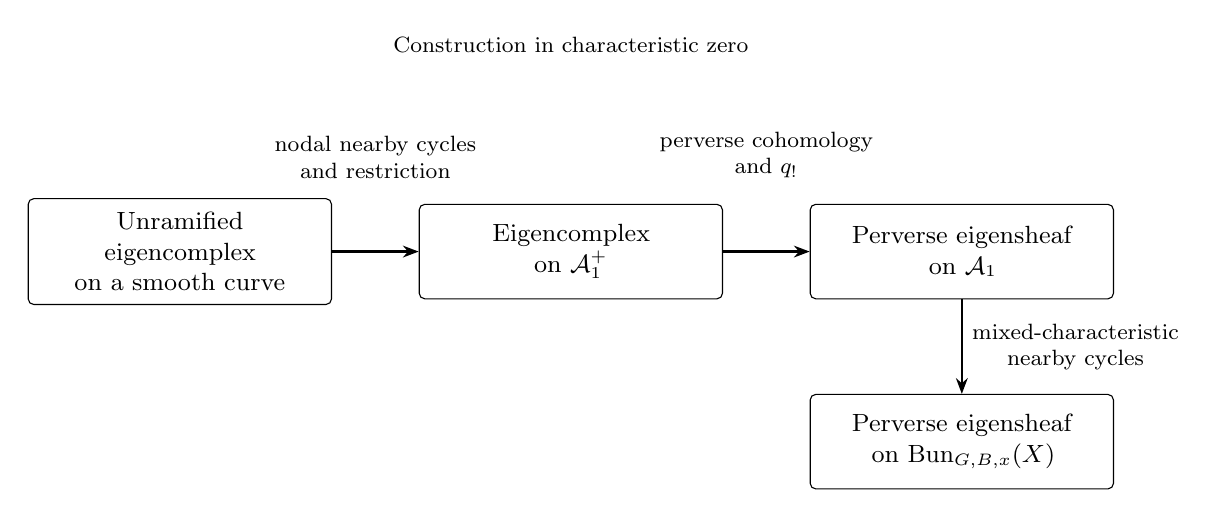
\begin{tikzpicture}[
 box/.style={draw,rounded corners=2pt,align=center,text width=3.5cm,
             minimum height=1.2cm,inner sep=5pt,font=\small},
 arr/.style={-{Stealth[length=2mm]},thick},
 lab/.style={font=\footnotesize,align=center}]
 \node[box] (unram) {Unramified eigencomplex\\on a smooth curve};
 \node[box,right=1.1cm of unram] (enh) {Eigencomplex\\on $\cA_1^+$};
 \node[box,right=1.1cm of enh] (ord) {Perverse eigensheaf\\on $\cA_1$};
 \draw[arr] (unram) -- node[lab,above=8mm]{nodal nearby cycles\\and restriction} (enh);
 \draw[arr] (enh) -- node[lab,above=8mm]{perverse cohomology\\and $q_!$} (ord);
 \node[lab,above=18mm of enh] {Construction in characteristic zero};
 \node[box,below=1.2cm of ord] (positive) {Perverse eigensheaf\\on $\Bun_{G,B,x}(X)$};
 \draw[arr] (ord) -- node[lab,right]{mixed-characteristic\\nearby cycles} (positive);
\end{tikzpicture}
\caption{The first specialization creates the level structure; the second
changes the characteristic. The arrow from enhanced to ordinary flags takes
perverse cohomology both before and after $q_!$. Each specialization also
requires a separate nonvanishing argument. The arrows record operations on
sheaves, not morphisms between the displayed moduli stacks.}
\label{fig:construction}
\end{figure}

The first difficulty is nonvanishing. Nearby cycles on a nonproper bundle
stack can annihilate a nonzero object; at the node they must also be
nonzero on the prescribed stabilizer type. Uniformization places a nonzero
generic stalk in a bounded Hecke space proper over a reference bundle of
that type. Its extension shows that the support approaches the required
special fiber. Theorem~\ref{thm:specialization-detection} then proves that
nearby cycles cannot vanish.

The detection arguments have a common local calculation but different
conclusions. Over a field, a nonnilpotent covector admits a transverse
Hecke modification with a nonzero moving-leg component. The two-Hecke
calculation and projective recovery use the lisse eigenrelation to show
that a function with that differential has zero vanishing cycles, excluding
the covector from singular support. Over a trait, assume that nearby cycles
vanish. The same local calculation forces nearby cycles to vanish on
hypersurface cuts whose differentials avoid the nilpotent cone. The cone
dimension bound allows enough simultaneous cuts to retain a nonzero generic
stalk while making the support finite over the trait. Its nearby cycles
are a nonzero sum of stalks, giving the contradiction. The two-Hecke and
projective slicing methods follow
\cite[Sections~3--7]{OpenAIFullSupport2026}; we prove their versions for
ordinary and enhanced Borel level and the simultaneous torus quotient,
under \ref{hyp:form}--\ref{hyp:nilpotent}.

Preserving the Hecke system requires more than commuting nearby cycles
with a fixed-point operator. The comparison must retain all moving legs,
including collisions, and the maps expressing convolution and fusion.
In input frames, each successive Hecke correspondence is a product with
a fixed Grassmannian Schubert model. The nearby-cycle exterior-product
comparison applies even when earlier modifications have made the input
singular. Iterating it and using proper convolution gives the entire
coherent system in Section~\ref{sec:specialization}.

Perverse cohomology presents a different issue: general Hecke functors
are not assumed to be perverse exact. Choose generators of the punctured
surface group. A framing of the parameter gives a monodromy tuple
$y\in Y=\Gd^{2g}$, whose simultaneous-conjugation orbit is closed and free
because the parameter is dense and $\Gd$ is adjoint. For each representation
$V$, the equivariant bundle $Y\times V$ admits an equivariant frame after
inverting an
invariant function $f_V$ nonzero at $y$. Under the Betti spectral action,
this frame identifies the fixed-point Hecke functor with $\dim V$ copies
of the identity wherever $f_V$ acts invertibly. The eigencomplex belongs
to this subcategory because $f_V$ acts on it by the scalar $f_V(y)$.
Inverting these functions gives a category stable under perverse
truncation, on which all fixed-point Hecke functors are exact.
Nadler--Yun's local constancy theorem extends this exactness to moving legs
and their collisions. Functorial truncation then preserves the original
eigenmaps and all their compatibilities (Section~\ref{sec:perverse}).

Finally, $q_!$ can vanish on an enhanced-flag object with arbitrary torus
monodromy. A central-sheaf trace identity relates that monodromy to the
boundary monodromy of the parameter. Unipotence of the latter forces
unipotence along the enhancement fibers and hence nonvanishing of $q_!$.
To globalize the trace identity, we retain independent input and output
enhancements during collision at the marked point. After removing the
contractible real radial directions of the enhancement torus, the bounded
pushforward is proper. This comparison preserves the monodromy on each
central factor, as the trace requires (Section~\ref{sec:descent}).

The geometric nearby-cycle foundations are those of
Hansen--Scholze \cite{HansenScholze} and Gaitsgory--Raskin \cite{GR}.
Throughout, finite reductions may require different finite trait
extensions; we do not replace them by one extension supporting the entire
adic system. All sheaves and parameters are geometric, and no Frobenius
structure is required.

Section~\ref{sec:foundations} fixes the sheaf and Hecke conventions.
Sections~\ref{sec:geometry} and~\ref{sec:detection} establish the cotangent
geometry and detection arguments. After the Hecke comparison, perverse
cohomology, and torus descent of
Sections~\ref{sec:specialization}--\ref{sec:descent},
Section~\ref{sec:construction} constructs the two families and assembles
the proof of Theorem~\ref{thm:main}.

\section{Sheaf conventions and the relative Hecke system}
\label{sec:foundations}

The argument will specialize sheaves twice and will use Betti sheaves in the
intermediate characteristic-zero fiber.  We first specify the sheaf categories
and the normalization in which these operations will be compared.  In
particular, the moving points of a Hecke correspondence contribute no shift to
the eigenvalue identity.

\subsection{Local constructibility and flag levels}

Write $E=\overline{\mathbb Q}_{\ell}$.  For a smooth algebraic stack $\cB$
locally of finite type over an algebraically closed field of characteristic
different from $\ell$, let $D_{\mathrm{lcc}}(\cB,E)$ denote the category of
geometric adic complexes whose pullback to every smooth finite-type scheme
chart is bounded and constructible.  The abbreviation ``lcc'' will always
mean \emph{locally bounded constructible}, not locally constant.  Bounds may
depend on the chart.  An object $F$ is perverse if
\[
                         f^*F[d]\in\operatorname{Perv}(D,E)
\]
for every smooth chart $f:D\to\cB$ of constant relative dimension $d$.
Charts of nonconstant relative dimension are treated componentwise.  This
defines the usual perverse $t$-structure locally and hence its truncations
and perverse cohomology on $D_{\mathrm{lcc}}$.  Neither this definition nor
the word ``perverse'' imposes a support condition on the set of
Harder--Narasimhan strata.

We use ordinary pullbacks and ordinary geometric stalks.  For a closed conic
subset $C\subset T^*\cB$, its pullback to a smooth chart is
\[
 f^{\circ}C
   =\operatorname{image}\bigl(D\mathbin{\times}_{\cB}C
                                      \longrightarrow T^*D\bigr).
\]
Thus $\SS(F)\subset C$ means $\SS(f^*F)\subset f^{\circ}C$ on every such
chart.  Shifting a complex does not change this condition.  The singular
support used here is the geometric adic singular support; existence and the
function-test characterization for bounded constructible $E$-complexes are
as in \cite[\S1.5, Theorem~(vii)]{Barrett}.

Fix a maximal torus in $B$ and identify it with $T=B/N_B$, where
$N_B=R_u(B)$.  For a smooth pointed projective curve $(X,x)$ put
\[
 \cA=\Bun_{G,B,x}(X),\qquad
 \cA^+=\Bun_{G,N_B,x}(X).
\]
An enhanced flag is an $N_B$-reduction of the fiber at $x$; forgetting the
enhancement gives a representable $T$-torsor
\begin{equation}\label{eq:found-level-torsor}
                             \pi:\cA^+\longrightarrow\cA.
\end{equation}
We also allow unlevelled bundles.  For two pointed curves with identified
flag tori, and a fixed choice of identification $\tau:T_1\simeq T_2$, write
\begin{equation}\label{eq:found-node-quotient}
 \cB_{12}=\bigl[(\cA_1^+\times\cA_2^+)/T_{\Delta}\bigr],
 \qquad T_{\Delta}=\{(t,\tau(t)):t\in T_1\}.
\end{equation}
The Borels on the two curves may be opposite.  The branch convention fixes
$\tau$ once and for all.  The map from $\cB_{12}$ to
$\cA_1\times\cA_2$ is a torsor under $(T_1\times T_2)/T_{\Delta}$.
An unramified Hecke modification on either punctured component transports
the level data and acts on the corresponding factor of this presentation.
Section~\ref{sec:geometry} describes the cotangent spaces and the
generic-nilpotence cone for all these stacks.

\subsection{Geometric specialization}

Let $S=\Spec R$ be an excellent complete strictly henselian discrete
valuation trait, with algebraically closed residue field $k$, and with
$\ell$ invertible in $R$.  Fix an algebraic closure $\overline K$ of its
fraction field.  Write $\bar\eta=\Spec\overline K$ and $s=\Spec k$.
For a finite-type $S$-scheme $Y$ we use geometric nearby cycles
\[
                \Psi_Y:D^b_c(Y_{\bar\eta},E)
                                  \longrightarrow D^b_c(Y_s,E).
\]
The geometric generic fiber is part of this notation.  In particular,
$\Psi_Y$ takes no inertia invariants.  When an object has descent data,
nearby cycles may retain the resulting inertia action, but the underlying
complex is the one used here.

It is useful to name the natural exchange maps.  For a morphism
$f:Y\to Z$ of models, and complexes $A,B$ on geometric generic fibers, they
are
\begin{align}
 \operatorname{Ex}^*_f &: f_s^*\Psi_Z A
                  \longrightarrow\Psi_Y(f_{\bar\eta}^*A),
                          \label{eq:found-pull-exchange}\\
 \operatorname{Ex}_{f,*} &: \Psi_Z(f_{\bar\eta,*}B)
                  \longrightarrow f_{s,*}\Psi_Y B,
                          \label{eq:found-push-exchange}\\
 \mu_{A,B} &: \Psi_Y A\otimes\Psi_Y B
                  \longrightarrow\Psi_Y(A\otimes B).
                          \label{eq:found-tensor-exchange}
\end{align}
We use the push exchange only where it is defined by the proper
nearby-cycle comparison, and therefore an isomorphism.  Pull exchange and
tensor exchange are not asserted to be isomorphisms in general.  For two
models $Y,Z$, their composite gives the exterior-product map
\begin{equation}\label{eq:found-exterior-exchange}
 \operatorname{Ex}^{\boxtimes}_{Y,Z}:
  \Psi_Y A\boxtimes\Psi_Z B
       \longrightarrow\Psi_{Y\times_S Z}(A\boxtimes B).
\end{equation}
The products in this formula are on the appropriate fibers of the product
over $S$.

\begin{proposition}[Geometric nearby-cycle formalism]
\label{prop:nearby-foundations}
For the traits just specified, geometric nearby cycles preserve bounded
constructibility and are exact for the perverse $t$-structures on the
geometric fibers.  They are unchanged by finite extension of the trait
inside $\overline K$.  The maps
\eqref{eq:found-pull-exchange}, \eqref{eq:found-push-exchange}, and
\eqref{eq:found-exterior-exchange} are isomorphisms, respectively, for
smooth $f$, for proper $f$, and for exterior products of bounded
constructible complexes.  These assertions extend to locally
constructible complexes on the smooth stacks used here by smooth descent;
proper morphisms in this extension are representable.

Let $L_{\bar\eta}$ be a lisse finite-rank $E$-sheaf on a model's geometric
generic fiber.  Suppose it has, after a finite extension of the coefficient
field, a lisse lattice whose finite reductions extend to lisse sheaves
after finite extensions of $S$.  Suppose these extensions are compatible
on further common extensions and have reductions of a lisse special-fiber
sheaf $L_s$.  The finite extension of $S$ may depend on the reduction.
Then, for any map $g:Y\to Z$ to that model and any
$F\in D^b_c(Y_{\bar\eta},E)$, the natural map is an isomorphism
\begin{equation}\label{eq:found-lisse-tensor}
  \Psi_Y F\otimes g_s^*L_s
       \xrightarrow{\ \sim\ }
             \Psi_Y(F\otimes g_{\bar\eta}^*L_{\bar\eta}).
\end{equation}
The statement also holds locally on the stacks in question, and is
compatible with tensor products and morphisms of the lisse systems.
\end{proposition}

\begin{proof}
We recall the coefficient issue because it prevents an unwarranted descent
hypothesis in the applications.  At torsion coefficient level, a
constructible object on $Y_{\bar\eta}$ descends to a finite extension of
$K$; the same holds for any specified finite diagram of objects and maps.
Geometric nearby cycles of those descents agree after further finite
extensions.  Hence the torsion functor is defined on the filtered union of
these categories, independently of all such choices.  Applying the adic
formalism and extension of coefficients gives the geometric functor above.
This construction is the specialization functor of
\cite[\S\S4.1.1--4.1.5]{GR}.  Different reductions of an adic object can
require different extensions of $K$; the construction does not replace this
tower by a single finite extension.

The constructibility and exchange assertions are recorded in
\cite[\S4.1.6]{GR}.  For the general traits used here, they follow from
\cite[Theorem~4.1 and Corollary~4.2]{HansenScholze}, in the rational-adic
coefficient setting~(C) of that paper.  Indeed, the integral closure $V$ of
$R$ in $\overline K$ is a rank-one absolutely integrally closed valuation
ring.  On a separated finitely presented $V$-scheme, restriction to the
generic fiber identifies universally locally acyclic complexes with
arbitrary constructible generic-fiber complexes; its inverse is $Rj_*$.
Nearby cycles are $i^*Rj_*$.  This applies to $E$ itself, and thus directly
to objects without common finite descent.  Perverse exactness follows
from this equivalence and the relative perverse $t$-structure of
\cite[Theorem~6.7]{HansenScholze}: generic restriction and special
restriction are exact for their fiberwise perverse structures.  Finite
extensions of the original trait give the same $V$.  On a smooth stack,
smooth pullback of relative dimension $d$
commutes with $\Psi$ and with $[d]$.  The scheme assertions therefore
descend, and give both local constructibility and perverse exactness on
the stack.  The proper assertion is checked after smooth base change to
schemes, or algebraic spaces, for a representable proper map.

For the last assertion choose the lattice and reduce modulo a power of its
uniformizer.  After the permitted trait extension its extension is lisse
on $Z$.  The lisse tensor formula for nearby cycles, after pullback to
$Y$, gives \eqref{eq:found-lisse-tensor} at this finite coefficient level.
Its construction is natural in reductions, maps, and further trait
extensions.  Passing to the adic system and then inverting the coefficient
uniformizer proves the assertion.  This proof permits arbitrary $g$:
it uses lisseness of the extended factor, not a base-change theorem for
$\Psi$ along $g$.
\end{proof}

All exchange maps above obey the following compatibilities.  Pull and
proper-push exchange compose for composite morphisms; tensor exchange is
associative and unital; and these maps commute with proper base change and
the projection formula.  They are the natural transformations obtained
from restriction and pushforward in the definition of nearby cycles, so
these identities hold before choosing any isomorphisms.  This observation
will identify the maps obtained by different orders of Hecke convolution.

\subsection{Relative Satake normalization}

For a dominant coweight $\lambda$, put
$d_\lambda=\langle2\rho,\lambda\rangle$.  The spherical Satake complex
$\IC_\lambda$ is normalized on the open Schubert orbit by
\begin{equation}\label{eq:found-satake-normalization}
               \IC_\lambda|_{\Gr^\lambda}
                         =E[d_\lambda](d_\lambda/2).
\end{equation}
Since $G$ is simply connected, its coweight lattice is the coroot lattice;
$\langle2\rho,\alpha^\vee\rangle=2$ for every simple coroot.  Thus every
$d_\lambda$ is even.  We choose the usual Satake equivalence with
$\Rep(\Gd)$, including its cohomological fiber functor and fusion
commutativity constraint; see \cite[\S\S4--6 and Theorem~14.1]{MV}.
Tate twists are geometric coefficient lines.  They require no Weil
structure, and compatible trivializations may be fixed in comparisons
with Betti coefficients.

Let $U$ be the smooth scheme locus of the curve on which modifications are
allowed, disjoint from all marked or stacky points.  For a finite set $I$,
let $\cH_I$ be the Beilinson--Drinfeld Hecke stack with input bundle map
$p_I$ and output-and-leg map
\[
                       o_I:\cH_I\longrightarrow\cB\times U^I.
\]
For representations $\boldsymbol V=(V_i)_{i\in I}$, let
$\operatorname{Sat}_I(\boldsymbol V)$ denote its relative spherical
kernel.  In input frames at pairwise distinct legs it is the exterior
product of the fixed-point Satake complexes, with normalization
\eqref{eq:found-satake-normalization}.  At collisions it is obtained by
the proper convolution map from successive modifications.  Define
\begin{equation}\label{eq:found-hecke-definition}
 \Hecke_{I,\boldsymbol V}(F)
   =o_{I,*}\bigl(F\,\widetilde\boxtimes\,
                                  \operatorname{Sat}_I(\boldsymbol V)\bigr).
\end{equation}
The twisted product is characterized in input frames by the ordinary
exterior product with $F$.  The equivariance of the Satake factor provides
its descent.  These formulas are computed on finite-dimensional bounds
containing the support of the kernel; the output map on each such bound
is representable and proper.  No shift $[|I|]$ occurs in
\eqref{eq:found-hecke-definition}.  In particular
\begin{equation}\label{eq:found-hecke-unit}
 \Hecke_{I,(\mathbf1)}(F)=F\boxtimes E_{U^I},\qquad \Hecke_{\varnothing}(F)=F.
\end{equation}
When discussing perversity over a smooth leg space, we will explicitly
insert $[|I|]$ and subsequently remove it.

For a surjection of finite sets $a:I\twoheadrightarrow J$, write
$\delta_a:U^J\to U^I$ for its collision diagonal, and put
$W_j=\bigotimes_{i\in a^{-1}(j)}V_i$.  The relative fusion convention is
\begin{equation}\label{eq:found-fusion}
  (1\times\delta_a)^*\Hecke_{I,\boldsymbol V}(F)
                         \simeq \Hecke_{J,\boldsymbol W}(F).
\end{equation}
There is no codimension shift in this ordinary-pullback formula.  The
usual shifts appear only if both sides have first been made perverse over
their respective leg spaces.  An eigenstructure throughout this paper
means natural isomorphisms for all $I$ and all representations, compatible
with these fusion maps, the unit, successive modifications, and
permutations.  A system of separate fixed-point eigenisomorphisms is not
sufficient.

\subsection{The use of Betti realization}

For a finite-type complex scheme, geometric adic constructible complexes
admit the usual realization as algebraically constructible complexes of
ordinary $E$-vector spaces on the analytic space.  It is obtained from
finite coefficient comparison and passage to adic coefficients; on a
lisse sheaf it restricts its continuous monodromy representation to
topological loops.  On bounded constructible objects the realization is
conservative, preserves the perverse $t$-structure, and commutes with the
pullbacks, tensor products, and finite-type pushforwards used below.  The
local finite-triangulation form of comparison ensures that these
operations commute with passage from a lattice to $E$-coefficients.
The characteristic-zero comparison convention is also used in
\cite[\S2.2.1]{GR}.

For algebraically constructible complexes this comparison identifies
algebraic singular support with the corresponding complex conic singular
support in the analytic cotangent bundle.  One can check the assertion
using the vanishing-cycle characterization: comparison identifies the
tests by algebraic functions, and such tests generate singular support.
We apply these statements on finite-type smooth charts and their
correspondence diagrams, and descend them to the stacks above.  In
particular Betti realization may verify that an already defined adic
truncation comparison is an isomorphism.  It does not create an adic
object from an arbitrary Betti object.  The infinite-rank universal
monodromic kernels appearing later are used only on the Betti side; all
objects subsequently specialized are geometric adic lcc complexes.

\section{Nilpotent cotangent cones and transverse modifications}
\label{sec:geometry}

The detection arguments require two geometric facts.  The nilpotent cone
must have at most half the dimension of the cotangent bundle on a smooth
chart, and a covector outside that cone must admit a Hecke modification
with a nonzero component in the direction of the moving point.  We prove
both facts, including the nondegeneracy of the modification that will be
needed for the slicing argument.

Throughout this section the ground field is algebraically closed.  It is
either of characteristic zero or is $k=\overline{\mathbb F}_q$, with the
four characteristic hypotheses of Theorem~\ref{thm:main}.  In characteristic
zero we choose an invariant form $\kappa$ with the same nondegeneracy
properties.  The stack $\cB$ will be an unlevelled bundle stack, a bundle
stack with ordinary or enhanced Borel level at one point, or, in
characteristic zero, the simultaneous torus quotient
$[(\cA_1^+\times\cA_2^+)/T]$ described in Section~\ref{sec:foundations}.
An actual Hecke modification is always made on one curve, away from its
marked point.

\subsection{Cotangent vectors and the dimension bound}

Let $\mathcal P$ be a $G$-bundle, with reduction to a subgroup $H$ at $x$,
where $H=B$ or $R_u(B)$, and put $\mathfrak h=\Lie(H)$.
The vector bundle governing its deformations is
the elementary modification
\[
 \mathcal E_H
 =\ker\bigl(\ad(\mathcal P)\longrightarrow
                  \ad(\mathcal P)_x/\mathfrak h\bigr).
\]
Its first cohomology is the space of infinitesimal deformations and its
zeroth cohomology is the infinitesimal automorphism space.  Serre duality
therefore identifies a degree-zero cotangent vector with a section
\begin{equation}\label{eq:geometry-cotangent}
 \phi\in H^0\bigl(X,\ad(\mathcal P)\otimes\omega_X(x)\bigr),
 \qquad \operatorname{Res}_x\phi\in\mathfrak h^\perp.
\end{equation}
Here and below a cotangent vector on a smooth stack means an element of
$H^0$ of the fiber of its cotangent complex.  Thus these descriptions
retain the infinitesimal automorphisms of the bundle stack; they do not
replace the stack by a coarse moduli space.

The $T$-weight decomposition and invariance of $\kappa$ show that opposite
root spaces pair perfectly and that $\kappa$ is nondegenerate on
$\mathfrak t$.  Consequently
\[
 \mathfrak b^\perp=\Lie R_u(B),\qquad
 (\Lie R_u(B))^\perp=\mathfrak b.
\]
Formula~\eqref{eq:geometry-cotangent} is thus the strongly parabolic
residue condition at ordinary level and the Borel residue condition at
enhanced level.  For the simultaneous torus quotient, its cotangent
vectors are pairs of enhanced-level Higgs fields annihilating the
infinitesimal diagonal torus action.  Under Serre duality the functional
on a change of enhancement is pairing with the toral component of the
residue, with the sign fixed by the action convention on that branch.

Write $\Lambda\subset T^*\cB$ for the cone of such fields that are
nilpotent over the function field of each curve.  It is closed: after
choosing homogeneous generators of the invariant polynomials, the
condition is the vanishing of their associated global sections.  The
identification of this zero fiber with generic nilpotence is valid under
Hypothesis~\ref{hyp:chevalley}.  Indeed an element can be conjugated into a Borel Lie
algebra, as also verified in the proof of
Lemma~\ref{lem:central-cocharacter} below; contraction of its nilradical
part leaves its toral part.  Restriction of invariants to the torus and
the finite Weyl group quotient then show that all positive-degree
invariants vanish exactly when that toral part is zero.  A finite-group
quotient separates its geometric orbits in every characteristic; no
averaging over the Weyl group is involved.

The residue of a generically nilpotent field is nilpotent.  For example,
in a parameter $t$ at $x$, write $\phi=b(t)\,dt/t$.  Every invariant
polynomial vanishes on $b(t)$ and hence on $b(0)$.  At enhanced level
$b(0)\in\mathfrak b$, so its toral projection vanishes.  It follows that
the enhanced-level cone is the smooth pullback of the ordinary-level
cone.  The same is true for the simultaneous torus quotient over
$\cA_1\times\cA_2$: both toral residues are already zero on its
nilpotent cone.  These assertions also describe the cones after
pullback to scheme charts.

\begin{proposition}\label{prop:cone-dimension}
Let $\cB$ be one of the bundle stacks just specified, and let
$f:D\to\cB$ be a smooth chart with $D$ a smooth finite-type scheme of
pure dimension $d$.  For the smooth cotangent pullback
$\Lambda_D=f^\circ\Lambda\subset T^*D$, one has
\begin{equation}\label{eq:geometry-cone-dimension}
                         \dim\Lambda_D\leq d.
\end{equation}
In characteristic zero this cone is isotropic, in the sense that the
symplectic form restricts to zero on the smooth locus of every reduced
subvariety of $\Lambda_D$.
\end{proposition}

\begin{proof}
We give the ordinary-level argument; the unlevelled version omits the
condition at $x$.  This is the parabolic form of the isotropy argument
for the global nilpotent cone \cite[Lemma~7]{GinzburgNilpotent}; compare the
separable-lifting criterion and its bundle-stack application in
\cite[Appendix~D.1.5 and D.1.8]{AGKRRV}.

Let $Z$ be an irreducible component of $\Lambda_D$ with its reduced
structure, and put $F=k(Z)$.  Its generic point specifies a family
$(\mathcal P,\beta,\phi)$ on $X_F$.  By
\cite[Theorem~2]{DrinfeldSimpson}, after a finite separable extension
$F'/F$ the bundle is trivial over the generic point of $X_{F'}$.
Hypothesis~\ref{hyp:nilpotent}, applied to the field $F'(X)$, gives a parabolic subgroup
whose nilradical contains the value of $\phi$ there.  In characteristic
zero the same assertion is the rational parabolic consequence of
Jacobson--Morozov.  Choose the standard parabolic $P$ of this type.
For the split group $G$, the scheme of parabolics of that type is
$G/P$; the rational parabolic therefore gives, in the generic
trivialization, a section of $\mathcal P/P$ over $F'(X)$.
This is the required generic $P$-reduction and does not require a
choice of rational conjugating element.  Properness of $G/P$ extends it to a reduction
$\mathcal Q$ on the whole smooth curve $X_{F'}$.  Since its nilradical
bundle is a subbundle of $\ad(\mathcal P)$, the generic containment
extends to
\[
 \phi\in H^0\bigl(X_{F'},
          \mathcal Q\mathbin{\times}^{P}\Lie R_u(P)
                     \otimes\omega_{X_{F'}}(x)\bigr).
\]

Consider the stack $\mathcal Y$ of a $P$-bundle together with a Borel
flag at $x$ in the relative position of $(\mathcal Q_x,\beta)$ just
obtained.  This stack is smooth.  Indeed $\Bun_P$ is smooth by the
vanishing of the second cohomology of its deformation bundle on a
curve, and the relative-position locus over it is the associated
bundle with fiber a $P$-orbit in $G/B$.  That orbit is smooth: its
stabilizer is an intersection of a parabolic and a Borel, with the
usual smooth torus and root-group description.

The pullback of $\phi$ to a cotangent vector on $\mathcal Y$ is zero.
To check this without suppressing the level condition, deformations
on $\mathcal Y$ are governed by the locally free sheaf $\mathcal E$
of sections of $\ad(\mathcal Q)$ whose value at $x$ lies in the
intersection with the Borel Lie algebra.  Pairing $\phi$ with
$\mathcal E$ has no pole at $x$, by the original residue condition.
It is zero generically because the nilradical of a parabolic is the
annihilator of its Lie algebra.  Hence the induced section of
$\mathcal E^*\otimes\omega$ is zero everywhere.  Serre duality proves
the asserted vanishing on deformation spaces.

Shrink to a smooth dense open of $Z$.  The finite separable extension
$F'/F$ spreads to a finite \emph{\'etale} cover of a smaller such open,
and the reduction spreads to a map from that cover to $\mathcal Y$.
The canonical one-form of $T^*D$ pulls back to zero there: it evaluates
the given covector on the induced deformation of the bundle, and this
deformation factors through $\mathcal Y$.  Since the cover is separable,
the one-form already vanishes on the smooth dense open of $Z$.
Its exterior differential, the symplectic form, also vanishes there.
An isotropic tangent space in $T^*D$ has dimension at most $d$, proving
\eqref{eq:geometry-cone-dimension}.  The separability in this argument
is essential; a purely inseparable cover would not detect vanishing
of differential forms.

Products and smooth pullbacks preserve this dimension bound: on
cotangent bundles a smooth pullback adds exactly the relative dimension
to the dimension of the cone.  The description of the enhanced and
quotient cones above therefore proves the remaining cases.  In
characteristic zero the same argument can start with any reduced
irreducible subvariety of the cone, rather than only an irreducible
component.  It gives the stated isotropy, which is likewise preserved
by products and smooth pullbacks.
\end{proof}

\subsection{A central cocharacter detecting a nonnilpotent value}

The modification below must be defined by an integral cocharacter.
Choosing merely an element of a toral Lie algebra would lose
information in positive characteristic.  The next lemma supplies an
actual cocharacter and the formal normal form needed for the residue
calculation.

\begin{lemma}\label{lem:central-cocharacter}
Over an algebraically closed field of characteristic zero, or over
$k=\overline{\mathbb F}_q$ under the four characteristic hypotheses,
let $a(t)\in\mathfrak g[[t]]$ with $a(0)$ not nilpotent.
After changing the formal $G$-frame, there are a Levi subgroup $M$ and
a cocharacter $\lambda:\mathbb G_m\to Z(M)$ such that
\begin{equation}\label{eq:geometry-levi-normal-form}
 \begin{gathered}
 a(t)\in\mathfrak m[[t]],\qquad
 \ad(a(0)):\mathfrak g/\mathfrak m\xrightarrow{\sim}
                                      \mathfrak g/\mathfrak m,\\
                         \kappa(a(0),d\lambda)\ne0.
 \end{gathered}
\end{equation}
Here $d\lambda$ is the image of $1\in\Lie\mathbb G_m$ under the
differential of $\lambda$.
\end{lemma}

\begin{proof}
We construct the Levi from the semisimple part of $a(0)$, choose a
central cocharacter that pairs nontrivially with that part, and then
remove the remaining off-Levi coefficients of the series.  The first
two steps require some care in positive characteristic.

\emph{The semisimple part and its centralizer.}
Embed $G$ as a
closed subgroup of some $\operatorname{GL}(W)$.  In positive
characteristic $\mathfrak g$ is closed under the restricted $p$-power,
which is matrix $p$-th power in this representation.  All eigenvalues
of $a(0)$ belong to a finite subfield of $k$.  For a sufficiently large
power $p^r$ that fixes these eigenvalues and kills every nilpotent
Jordan block, matrix power $a(0)^{p^r}$ is its semisimple part $s$.
Consequently both $s$ and $n=a(0)-s$ belong to $\mathfrak g$ and
$[s,n]=0$.  In characteristic zero this is the usual Jordan
decomposition in an algebraic Lie algebra.

To identify $s$ and $n$ intrinsically, fix a maximal torus $T$, a simple system
$\Delta$, and compatible root vectors $e_\alpha,e_{-\alpha}$ with
$[e_\alpha,e_{-\alpha}]=d\alpha^\vee$.  Invariance gives
\begin{equation}\label{eq:geometry-root-pairing}
 \kappa(d\alpha^\vee,H)=c_\alpha\,d\alpha(H),
 \qquad c_\alpha=\kappa(e_\alpha,e_{-\alpha})\ne0
 \quad(H\in\mathfrak t).
\end{equation}
The nonzero constant follows from the perfect pairing of opposite
$T$-weight spaces.  Hypothesis~\ref{hyp:form}, applied to the Levi $T$, makes
$\kappa|_{\mathfrak t}$ nondegenerate.  Since $G$ is simply connected,
the simple coroots form a basis of $X_*(T)$; their differentials are
therefore a basis of $\mathfrak t$.  Equation~\eqref{eq:geometry-root-pairing}
shows that the simple-root differentials are linearly independent.
The same equation, applied to any root, shows that its differential
is nonzero.

We claim that matrix semisimplicity agrees with the toral definition
in the theorem, and that matrix nilpotence agrees with the orbit-closure
definition.  The proper incidence morphism
\[
             G\mathbin{\times}^{B}\mathfrak b\longrightarrow\mathfrak g
\]
is surjective.  Its differential is surjective at a toral element
outside the finitely many root-differential hyperplanes, so its closed
image contains a dense open.  Inside $\mathfrak b$, write an element
as $H+u$.  Successive conjugations by root groups, in increasing root
height, remove every root coefficient with $d\alpha(H)\ne0$:
the coefficient in question changes by a nonzero multiple of the
root-group parameter, while changes to other coefficients occur in
higher heights.  The remaining term $u_0$ commutes with $H$ and is a
nilpotent matrix.  Thus $H+u_0$ is matrix semisimple only if $u_0=0$.
Likewise a matrix nilpotent in $\mathfrak b$ has zero toral projection,
since a faithful representation is upper triangular on $B$ and its
toral differential is injective.  Contraction by a strictly dominant
cocharacter sends the nilradical to zero.  This proves that matrix
nilpotence is equivalent to the orbit-closure definition; the reverse
implication also follows directly from the closed matrix nilpotent
cone.  The same argument applies inside any Levi.

We may now conjugate $s$ into $\mathfrak t$.  Since $a(0)$ is not
nilpotent, $s\ne0$.  Hypothesis~\ref{hyp:centralizer} makes its scheme-theoretic
centralizer a Levi $M=Z_G(s)$.  We have
$s\in\mathfrak z(\mathfrak m)$ and $n\in\mathfrak m$.
Conjugate $n$ within $M$ into a Borel nilradical of $\mathfrak m$,
using the preceding argument.  Torus weights then show that $n$ is
orthogonal to $\mathfrak z(\mathfrak m)$; this conclusion is unchanged
by the conjugation.

\emph{Choosing an integral central cocharacter.}
To detect $s$ by a cocharacter, we need the differentials of central
cocharacters to span $\mathfrak z(\mathfrak m)$.  We verify this before
using the nondegeneracy of $\kappa$ on the center.
Choose the simple system $\Delta$ so that $M$ corresponds to a subset
$\Delta_M\subset\Delta$.
Its Lie center is
\[
 \mathfrak z(\mathfrak m)
       =\bigcap_{\alpha\in\Delta_M}\ker(d\alpha)\subset\mathfrak t.
\]
There are no additional central root vectors, since each root
differential is nonzero.  The integral map
\[
 X_*(T)\longrightarrow\mathbb Z^{\Delta_M},
 \qquad \nu\longmapsto
                 (\langle\alpha,\nu\rangle)_{\alpha\in\Delta_M}
\]
has full row rank after reduction modulo $p$ in positive characteristic,
by the linear independence of the simple-root differentials proved above.
Its Smith normal form therefore has no nonunit elementary divisor
divisible by $p$.
It follows that the kernel of its differential is spanned over $k$
by the differentials of its integral kernel.  The latter kernel is
exactly $X_*(Z(M))$.  Thus the Lie center is spanned by differentials
of actual central cocharacters.  In characteristic zero the same
conclusion follows by tensoring the integral kernel with $k$.

By Hypothesis~\ref{hyp:form} the restriction of $\kappa$ to
this center is nondegenerate, and by the integral-kernel calculation
its central cocharacter differentials span it.  Some
$\lambda\in X_*(Z(M))$ therefore satisfies
\[
             \kappa(a(0),d\lambda)
                    =\kappa(s,d\lambda)\ne0.
\]
On $\mathfrak g/\mathfrak m$ the operator $\ad(s)$ is invertible and
$\ad(n)$ is nilpotent and commutes with it.  Their sum is invertible,
giving the middle assertion of
\eqref{eq:geometry-levi-normal-form}.

\emph{Putting the formal series in the Levi.}
It remains to put the whole series in $\mathfrak m[[t]]$.  Decompose
$\mathfrak g$ into the zero and nonzero eigenspaces of $\ad(s)$,
so that the first summand is $\mathfrak m$.  Suppose inductively that
the non-$\mathfrak m$ coefficients below order $t^r$ have been removed.
Conjugation by a group element congruent to $1+t^rY$ modulo $t^{r+1}$
changes the offending coefficient by $[Y,a(0)]$.  The invertibility
just proved supplies $Y$ that removes it.  Such a group element exists
by smoothness of $G$.  The successive changes converge in $G(k[[t]])$,
proving the first assertion without changing the constant term.
\end{proof}

\subsection{The two tangent maps of a Hecke modification}

The central-cocharacter modification below follows the microlocal method of
\cite[Sections~20.5 and~20.7--20.8]{AGKRRV} and the transverse formulation
in \cite[Proposition~4.2]{OpenAIFullSupport2026}. We include both tangent
calculations, since the slicing argument uses them on opposite fibers.

Let $U$ denote the allowed moving-point curve, or the disjoint union of
the two allowed curves in the quotient case.  An exact-relative-position
Hecke correspondence $H$ has maps
\[
 p:H\longrightarrow\cB,\quad o:H\longrightarrow\cB,\quad
 \operatorname{leg}:H\longrightarrow U,
 \qquad q=(o,\operatorname{leg}),\quad
 \widetilde p=(p,\operatorname{leg}).
\]
Thus $p$ remembers the input bundle and $o$ the output bundle.
For relative position $\lambda^+$, both $q$ and $\widetilde p$ are
representable smooth of relative dimension
$m=\langle2\rho,\lambda^+\rangle$.  This is the usual smooth
affine-Grassmannian orbit description in disc frames.  Its Schubert
closure is a bound proper over either bundle together with the leg;
the inverse modification gives the description from the other side.
These facts hold in families of smooth legs, and a level condition at
a disjoint point is transported unchanged.

\begin{proposition}\label{prop:transverse-hecke}
Let $A\in T^*_{b}\cB$ be a covector outside $\Lambda$.  There exist a
point $y\in U$, an exact-relative-position correspondence $H$, a
modification $h\in H$ with $p(h)=b$ and leg $y$, an output covector
$A'\in T^*_{o(h)}\cB$, and a nonzero $\xi\in T^*_yU$ such that
\begin{equation}\label{eq:geometry-covector-identity}
                         p^*A=q^*(A',\xi)\quad\text{at }h.
\end{equation}
Put
\[
 H_{\mathrm{in}}=\widetilde p^{-1}(b,y),\qquad
 H_{\mathrm{out}}=q^{-1}(o(h),y),
\]
where the fibers include the fixed-side bundle identifications.  Both
are smooth of dimension $m$.  The following two sections have
nondegenerate zeros at $h$:
\begin{enumerate}
\item on $H_{\mathrm{in}}$, the restriction of $p^*A$ to
      $T_{H/(\cB\times U),q}|_{H_{\mathrm{in}}}$;
\item on $H_{\mathrm{out}}$, the restriction of $o^*A'$ to
      $T_{H/(\cB\times U),\widetilde p}|_{H_{\mathrm{out}}}$.
\end{enumerate}
Each is a section of the dual of the indicated rank-$m$ bundle.
In particular, both zeros are isolated.
\end{proposition}

\begin{proof}
Represent $A$ by its Higgs field or pair of fields.  On a curve where
it is not generically nilpotent, choose an unmarked point $y$ at which
the value is not nilpotent.  In a parameter $t$ centered at $y$ and a
formal frame, write this field as $a(t)\,dt$.
Lemma~\ref{lem:central-cocharacter} supplies $M$ and $\lambda$ satisfying
\eqref{eq:geometry-levi-normal-form}.  Make the modification by
$\lambda(t)$, with the convention that its adjoint output lattice is
\[
 L'=\operatorname{Ad}(\lambda(t))L,
 \qquad L=\mathfrak g[[t]],\qquad J=L\cap L'.
\]
Because $\lambda$ centralizes $M$, the field $a(t)\,dt$ is regular in
both lattices.  It therefore transports to a global output covector
$A'$ with the same residue conditions at every marked point.

We record explicitly the tangent spaces and their pairing.  Gauge
transformations on the input formal disc move $L'$, whereas those on the output
move $L$.  Quotienting in each case by the common stabilizer gives
\begin{equation}\label{eq:geometry-two-tangents}
 T_hH_{\mathrm{in}}=L/J,
 \qquad T_hH_{\mathrm{out}}=L'/J.
\end{equation}
Both $L$ and $L'$ are their own annihilators for the pairing
$\operatorname{Res}_{t=0}\kappa(-,-)\,dt$.  More explicitly, if
$\mathfrak g=\bigoplus_{j\in\mathbb Z}\mathfrak g_j$ is the
\emph{integer} weight decomposition for $\lambda$, then
\begin{equation}\label{eq:geometry-truncated-lattices}
 \begin{aligned}
 L/J&=\bigoplus_{j>0}
           \mathfrak g_j\otimes k[[t]]/(t^j),\\
 L'/J&=\bigoplus_{j<0}
           \mathfrak g_j\otimes t^jk[[t]]/k[[t]].
 \end{aligned}
\end{equation}
Opposite weights pair perfectly under $\kappa$, and the coefficient
of $t^i$ pairs with that of $t^{-1-i}$.  Thus
\begin{equation}\label{eq:geometry-residue-perfect}
 (L/J)\times(L'/J)\longrightarrow k,
 \qquad (D,C)\longmapsto\operatorname{Res}\kappa(D,C)\,dt
\end{equation}
is a perfect pairing of $m$-dimensional vector spaces.

To compute the covector identity, first hold the output and leg fixed.
A tangent vector represented by $C\in L'$ changes the input bundle
by that principal part.  Serre duality evaluates $p^*A$ on it as
$\operatorname{Res}\kappa(a(t),C)\,dt$, which vanishes because
$a(t)\in L'$.  The degree-zero smooth cotangent exact sequence for
$q$ implies that $p^*A$ is the pullback of a covector on output bundle
times leg.  This argument is valid for stack covectors: the pullback
in that exact sequence is injective, and its image consists precisely
of covectors annihilating the relative tangent space.

The bundle component is $A'$.  It can be tested on principal parts
at points away from $y$ and the markings, where the input and output
are identified.  Such tests span the deformation space: sufficiently
large pole divisors supported at those points kill the first
cohomology of the deformation bundle, and the principal-parts exact
sequence then surjects onto that first cohomology.  For the moving-point
component, hold the output fixed and replace $t$ by $t-z$ in the
modification.  The logarithmic derivative of $\lambda(t-z)$ at $z=0$
is $-d\lambda/t$.  Consequently, up to the common sign determined by
the gluing convention,
\begin{equation}\label{eq:geometry-leg-covector}
                 \xi=\pm\kappa(a(0),d\lambda)\,dz\ne0.
\end{equation}
These computations prove \eqref{eq:geometry-covector-identity}.
In the simultaneous quotient case they may first be made with both
enhancements retained and then descended along the smooth torus
quotient; the modified curve is disjoint from all gluing data.

It remains to prove the two nondegeneracy assertions.  The perfect
pairing above pairs tangents to the two fixed-side fibers; its
$\ad(a(t))$-twist will be the derivative of each section.
Move in $H_{\mathrm{in}}$ in direction $D\in L/J$ and transport a
test vector $C\in L'/J$ with the moving lattice.  Differentiating its
pairing with the fixed input covector gives
\begin{equation}\label{eq:geometry-derivative-pairing}
 \operatorname{Res}\kappa(a(t),[D,C])\,dt
       =\operatorname{Res}\kappa([a(t),D],C)\,dt,
\end{equation}
up to the same harmless choice of sign.  The expression is independent
of lifts of $D$ and $C$: $\ad(a(t))$ preserves $L$, $L'$ and $J$.
It preserves every $\lambda$-weight space because
$a(t)\in\mathfrak m[[t]]$ and $\lambda$ is central in $M$.
For $j\ne0$, $\mathfrak g_j$ lies in the noncentralizer summand
$\mathfrak g/\mathfrak m$; hence the constant term of this operator
is invertible on $\mathfrak g_j$.  It is therefore invertible on
each of the truncated modules in
\eqref{eq:geometry-truncated-lattices}.  The perfect residue pairing
\eqref{eq:geometry-residue-perfect} makes
\eqref{eq:geometry-derivative-pairing} perfect as well.  This is exactly
the derivative of the first section in the statement at its zero.

For the section on $H_{\mathrm{out}}$, keep the output fixed, move
$L$ using $C\in L'/J$, and transport $D\in L/J$.  The resulting derivative is
the transpose of \eqref{eq:geometry-derivative-pairing}, up to sign.
It too is perfect.  A section of a rank-$m$ vector bundle on a smooth
$m$-dimensional fiber whose derivative at a zero is invertible has
an isolated reduced zero there, proving both assertions.  All
truncation lengths in this proof are integer cocharacter weights;
none is inverted in $k$.
\end{proof}

The two fibers will have different roles in the detection argument.
The nondegenerate zero on $H_{\mathrm{out}}$ isolates a contribution
to a proper Hecke pushforward.  The zero on $H_{\mathrm{in}}$ supplies
the coordinates transverse to that contribution and yields the exact
split quadratic equation of Section~\ref{sec:detection}.

\section{Hecke eigencomplexes and transverse slices}\label{sec:detection}

We now turn the transverse modification of
Proposition~\ref{prop:transverse-hecke} into a sheaf-theoretic detection
argument.  There are two conclusions.  Over a field, a Hecke eigencomplex
has singular support in the generically nilpotent cone.  Over a trait, a Hecke
eigencomplex cannot have zero nearby cycles if its support approaches the
special fiber.  The same two-Hecke correspondence proves both statements;
the final step of the second also uses the dimension bound of
Proposition~\ref{prop:cone-dimension}.
The moving-leg argument and the isolation of a covector by a modification
have close predecessors in \cite[\S\S20.5--20.8]{AGKRRV}; their
vanishing-cycle method also uses transverse quadratic functions
\cite[Appendix~H, especially Remark~H.2.5]{AGKRRV}. The two-modification
quadratic model and the projective slicing arguments are the unramified
methods of \cite[Proposition~5.1, Section~6, and Lemma~7.2]{OpenAIFullSupport2026}.
We prove their field and trait versions here for the level stacks required
in the construction. A projective quadric calculation recovers the original
hypersurface from the local model supplied by the two modifications.

Throughout this section, a bundle stack over an algebraically closed field
means one of the stacks considered in Section~\ref{sec:geometry}: the
unlevelled bundle stack on a smooth projective curve, the bundle stack with
ordinary or enhanced Borel level at a marked point, or, in characteristic
zero, the quotient of two enhanced-level bundle stacks by the simultaneous
flag torus.  In the last case Hecke modifications act separately on the two
punctured curves.  We write $\cB$ for the stack and $\Lambda\subset T^*\cB$
for its cone of Higgs fields generically nilpotent on every curve.  For a
smooth scheme chart $b:D\to\cB$, $\Lambda_D$ denotes the image of the
pullback of this cone under the cotangent map.  The group and characteristic
hypotheses are those of Section~\ref{sec:geometry}.

\begin{theorem}[Nilpotent detection]\label{thm:nilpotent-detection}
Let $\cB$ be such a bundle stack over an algebraically closed field, and
let $F$ be a locally bounded constructible $E$-complex on $\cB$.  Suppose
that, for every spherical Satake representation $V$ and each curve on
which modifications are allowed, there is an isomorphism
\[
                  \Hecke_V(F)\simeq F\boxtimes\mathcal V_V
\]
with $\mathcal V_V$ lisse on the open curve.  Then
$\SS(b^*F)\subset\Lambda_D$ for every smooth finite-type scheme chart
$b:D\to\cB$.
\end{theorem}

The specialization statement uses the following precise relative setup.
Let $S=\Spec R$ be an excellent complete strictly henselian trait on which
$\ell$ is invertible, with
algebraically closed residue field, generic point $\eta$, and geometric
generic point $\bar\eta$.  Let $\cB\to S$ be smooth and locally of finite
type, with special fiber one of the preceding bundle stacks.  Assume that
there is a smooth scheme of legs $L\to S$ of relative dimension one,
whose special fiber contains a nonempty open subset of every allowed
special-fiber curve, with the usual
spherical Hecke correspondences.  Their bounded output maps to
$\cB\times_S L$ are representable and proper.  Each exact-relative-position
stratum is smooth over $(\text{input bundle},\text{leg})$ and over
$(\text{output bundle},\text{leg})$, and has the special-fiber geometry of
Proposition~\ref{prop:transverse-hecke}.  The Satake kernel on its open
stratum is the constant sheaf with its relative Satake shift and twist.
These conditions hold for the pointed smooth family and for the twisted
nodal family used below.

\begin{theorem}[Specialization detection]\label{thm:specialization-detection}
In this relative setup, let $F$ be a locally bounded constructible
$E$-complex on $\cB_{\bar\eta}$ with lisse Hecke eigenvalues on
$L_{\bar\eta}$.  Suppose each eigenvalue admits a lisse lattice whose
finite reductions extend lisse after finite extensions of the trait,
compatibly with its special-fiber value, as in
Proposition~\ref{prop:nearby-foundations}.  If $\Psi F=0$, then, on every
smooth finite-type chart $D\to\cB$, the closure of the nonzero-stalk locus
of $F|_{D_{\bar\eta}}$ does not meet $D_s$.
Equivalently, any such meeting forces $\Psi F\ne0$.
\end{theorem}

The closure in this statement can be computed after descending its finitely
many geometric generic components to a finite extension of $R$.  It does
not require a field of definition for $F$ itself.  All extensions below are
taken inside the fixed geometric generic field.  Nearby cycles always mean
geometric nearby cycles, without inertia invariants.

\subsection{A hypersurface cut and two Hecke modifications}

The common step in the two theorems is a calculation for one hypersurface.
We keep the two coefficient complexes distinct.  In the \emph{field case},
let $F$ satisfy the hypotheses of Theorem~\ref{thm:nilpotent-detection},
take a smooth chart $b:D\to\cB$, a closed point $d$, and a regular function
$f$ near $d$ with $f(d)=0$, and put $K=b^*F$.
Here $L$ is the open curve of allowed legs, or the disjoint union of the
two open curves in the quotient case.  In the \emph{trait case}, let $F$
satisfy the hypotheses of Theorem~\ref{thm:specialization-detection}
and assume $\Psi F=0$.  Take a smooth chart $b:D\to\cB$ over $S$,
a closed point $d\in D_s$, and a regular function $f$ with $f(d)=0$;
put $K=b_{\bar\eta}^*F$.  Thus $K$ is defined on $D$ in the field case
and only on $D_{\bar\eta}$ in the trait case.

\begin{lemma}[Hypersurface calculation]\label{lem:detection-hypersurface}
If the differential $df_d$ in the field case, respectively its relative
special-fiber differential in the trait case, lies outside $\Lambda_D$,
then
\[
      (\Phi_f K)_d=0
      \quad\text{in the field case},\qquad
      \bigl(\Psi(K|_{\{f=0\}_{\bar\eta}})\bigr)_d=0
      \quad\text{in the trait case}.
\]
Here $\Phi_f$ is the unshifted cone from restriction to geometric nearby
cycles for $f$.
\end{lemma}

\begin{proof}
The Hecke eigenrelation first gives a vanishing after proper pushforward.
The two nondegenerate zeros of Proposition~\ref{prop:transverse-hecke}
then have different roles: one isolates a single stalk in that pushforward,
and the other gives local coordinates in which the equation is the original
hypersurface equation plus a split quadratic form.  A projective compactification
will recover the cycles of the original hypersurface from those of the
stabilized one.

\smallskip\noindent
\emph{1. The modified hypersurface and the eigenrelation.}
If $df_d$ is nonzero on the tangent space relative to $b$, the map
$(b,f):D\to\cB\times\mathbb A^1$ is smooth near $d$ in the field case,
and $\{f=0\}\to\cB$ is smooth near $d$ in the trait case.  Smooth base
change proves the assertion.  We may therefore assume
$df_d=b^*A$ for a covector $A\notin\Lambda$ at $b(d)$.

Choose the modification $h$ supplied by
Proposition~\ref{prop:transverse-hecke}, at a leg $y$.  Write $H$ for its
exact-position Hecke stratum and
\[
 p:H\longrightarrow\cB,\qquad
 o:H\longrightarrow\cB,\qquad
 q=(o,\operatorname{leg}):H\longrightarrow\cB\times L,
 \qquad \widetilde p=(p,\operatorname{leg}).
\]
Both $q$ and $\widetilde p$ are smooth of relative dimension $m$.  At $h$
the proposition gives
\begin{equation}\label{eq:detection-leg}
                 p^*A=q^*(A',\xi),\qquad \xi\ne0.
\end{equation}
Use the two fibers named in that proposition:
\[
 H_{\mathrm{in}}=\widetilde p^{-1}(b(d),y),\qquad
 H_{\mathrm{out}}=q^{-1}(o(h),y).
\]
On $H_{\mathrm{in}}$, the restriction of $p^*A$ to the $q$-relative
tangent has a nondegenerate zero at $h$; on $H_{\mathrm{out}}$, the
restriction of $o^*A'$ to the $\widetilde p$-relative tangent does too.
Each fiber retains the identification with its fixed-side bundle.

In the trait case these are special-fiber statements; take the
corresponding relative Hecke stratum over $S$.  In the field case introduce
the trait in the function line with parameter $z$, extend all spaces
constantly, and impose $f=z$.  We will apply vanishing cycles over this
trait.  Thus the two cases have a common notation: $e=0$ in the trait
case and $e=z$ in the field case, and the operation to be computed is,
respectively, $\Psi$ and $\Phi$.

Take two copies $H_1,H_2$ of $H$ and form
\begin{equation}\label{eq:detection-double}
 W_0=H_2\times_{p,\cB}D,
 \qquad
 P=H_1\times_{q,\cB\times L,q}W_0.
\end{equation}
Thus the two modifications have the same output bundle and leg, while
the input of the second lies in the chart $D$.  The defining square is
\[
\begin{CD}
 P @>{\operatorname{pr}_1}>> H_1\\
 @V{\operatorname{pr}_2}VV @VV{q}V\\
 W_0 @>{q_2}>> \cB\times L,
\end{CD}
\qquad
 W_0\longrightarrow D\longrightarrow\cB,
\]
where $q_2$ is the output-and-leg map of the second modification and the
composite on the right is its input map.
Let $c:P\to D$ be the projection through $W_0$.  Set
$W=\{f=e\}\subset W_0$ and $P_c=\{f(c)=e\}\subset P$.
The distinguished points are $w=(h,d)$ in $W_s$ and
$a=(h,h,d)$ in $(P_c)_s$.  Products here are over the trait when one is
present.

The output-bundle map $W\to\cB$ is smooth near $w$.  Indeed,
$W_0\to\cB\times L$ is smooth, and
\eqref{eq:detection-leg} says that the cut differential, on directions
relative to the output bundle, has the nonzero leg component $\xi$.
The eigenisomorphism therefore implies that the cycles of the pulled-back
Hecke transform vanish at $w$.  In the trait case this is smooth base
change from $\Psi F=0$, followed by the lisse tensor compatibility.  In
the field case $W\to\cB_S$ is smooth over the function trait, where
$\cB_S$ is the constant stack.  Pullback of the constant family with
coefficient $F$ therefore has zero vanishing cycles, and tensoring by
the lisse eigenvalue preserves this assertion.  The map to the bundle
stack is what is smooth here; no smoothness of
$W\to\cB\times L$ is needed.

\smallskip\noindent
\emph{2. Isolating one stalk in the proper pushforward.}
Replace $H_1$ in \eqref{eq:detection-double} by its proper Schubert bound
$\overline H_1$.  Choose the Satake representation whose kernel is the
intersection complex of this bound.  Proper base change identifies the
cycles of the preceding transform with the proper push of the cycles of
its Satake integrand.  If $T$ is the proper fiber over $w$ and $C$ is the
restriction of those cycles to $T$, we obtain
\begin{equation}\label{eq:detection-proper-zero}
                            R\Gamma(T,C)=0.
\end{equation}
We next isolate the contribution of $a$; no assertion about the boundary
of the Schubert variety is required.
In the field case the Satake integrand is defined on the entire constant
family and then restricted to the cut $f(c)=z$; $C$ is the restriction
of its vanishing cycles.  In the trait case we instead start with the
geometric-generic integrand and take its nearby cycles.

Before cutting, $P\to\cB$ by the first input bundle is smooth.  At a
point of $T$ in its open-orbit neighborhood, failure of smoothness after
cutting would mean that $d(f\circ c)$ comes from the cotangent space of
that first input bundle.  On this fiber the same differential is the
pullback of $(A',\xi)$ along $q_1$.  Since $P\to H_1$ is smooth, its
cotangent map is injective; thus failure would already give on $H_1$
an equality
\[
                         q_1^*(A',\xi)=p_1^*A_1
\]
for some $A_1$.  On $\widetilde p_1$-relative tangents this forces
$o_1^*A'$ to vanish.  The nondegenerate zero on $H_{\mathrm{out}}$
shows that $a$ is isolated among such points of $T$.  Consequently $C$
vanishes on a punctured neighborhood of $a$ in $T$: there the cut map
to the first input stack is smooth and the open-orbit Satake kernel is
an invertible constant shift and twist.
This smoothness is over the trait.  In the field case the integrand
therefore pulls back the constant $F$-family on $\cB_S$, so it has zero
$\Phi$, as required; the trait case uses $\Psi F=0$.
Here the open part of $T$ is exactly $H_{\mathrm{out}}$ for $H_1$,
since $w$ fixes the second modification and $d$.

Here is the precise consequence of this isolation.  If a constructible
complex on a proper scheme vanishes on a punctured neighborhood of a
closed point, its contribution at that point is a direct summand of its
global cohomology.  To see this, let $j:T\setminus\{a\}\to T$ and
$i:\{a\}\to T$.  The restriction $j^*C$ is zero near $a$, so
$(Rj_*j^*C)_a=0$.  The localization triangle consequently splits as the
direct sum of $i_*C_a$ and $Rj_*j^*C$; both connecting morphisms vanish
by these disjoint supports.  The same localization argument applies
to algebraic spaces.  Equation
\eqref{eq:detection-proper-zero} now gives
\begin{equation}\label{eq:detection-vertex-zero}
                                  C_a=0.
\end{equation}

\smallskip\noindent
\emph{3. An exact split quadratic equation at the isolated point.}
We identify the local equation at this isolated point exactly.  The
diagonal $W_0\to P$, given by making the two modifications equal, is a
section of the smooth map $P\to W_0$.  Etale locally at $a$, there is a
map $r:P\to D$ lifting the first-input map to $\cB$, whose restriction
to this diagonal is the original chart point, including its
identification with the first input.  Indeed, the smooth morphism
$P\times_{\cB}D\to P$ has that section on the diagonal.  To extend it,
choose relative smooth coordinates, giving an etale map from a
neighborhood of its value to $\mathbb A^\delta_P$, where $\delta$ is
the relative dimension of $D\to\cB$ at $d$.  The coordinates of the
prescribed section are functions on the diagonal; lift these functions
to a neighborhood in $P$ and take their graph in $\mathbb A^\delta_P$.
Pullback of the etale map along this graph gives an etale neighborhood
of $P$ with a lift to $P\times_{\cB}D$.  Retain the branch carrying
the prescribed section along the diagonal.  The resulting projection
to $D$ is $r$, and the fiber product retains the specified stack
isomorphism between $b\circ r$ and the first input.
Thus $c$ records the second input everywhere, whereas $r$ records the
first input in this etale neighborhood; the two agree on the diagonal.
The diagonal, being a section of the smooth morphism $P\to W_0$ of
relative dimension $m$, is a regular immersion of codimension $m$.
Choose relative coordinates $v_1,\ldots,v_m$ generating its ideal.
Since $r=c$ on it, there are functions $u_i$ with
\begin{equation}\label{eq:detection-exact-uv}
                         f(c)-f(r)=\sum_{i=1}^m u_i v_i.
\end{equation}
This is an equality of functions, not merely an equality of quadratic
terms.

On the diagonal fiber with $c=d$ and leg $y$, which is the fixed-input,
fixed-leg fiber of $H$ through $h$, the conormal coefficients
$u_i$ are the negatives of the restriction of $p^*A$ to the
$q$-relative tangent, in the frame dual to the $v_i$.  In fact variation
of the first modification with the second fixed has $dc=0$, whereas
$b\circ r$ is its first input, so differentiating
\eqref{eq:detection-exact-uv} gives precisely this restriction.  This
calculation is independent of the chart-vertical part of $dr$:
$df_d=b^*A$ annihilates $\ker(db_d)$.
The description holds along that entire diagonal fiber.  The
nondegenerate zero on $H_{\mathrm{in}}$ shows that $u_i(a)=0$ and that the
derivatives of the $u_i$ on that fiber form a basis.  The map
$W_0\to D\times L$ is the smooth base change of $\widetilde p$,
of relative dimension $m$.  On the diagonal,
$r=c$ and the leg provide the other coordinates; the $v_i$ provide its
normal coordinates.  Hence
\begin{equation}\label{eq:detection-uv-chart}
 (r,\operatorname{leg},u_1,\ldots,u_m,v_1,\ldots,v_m):
 P\longrightarrow D\times L\times\mathbb A^{2m}
\end{equation}
is etale near $a$, with the evident relative interpretation over $S$.
The first-input integrand is $r^*K$ up to its invertible constant shift
and twist.  Thus \eqref{eq:detection-vertex-zero} says that its cycles
vanish at the vertex of
\begin{equation}\label{eq:detection-affine-quadric}
                         f+\sum_i u_i v_i=e.
\end{equation}
For $m=0$ this is already the required assertion, after removing the
smooth leg factor.

\smallskip\noindent
\emph{4. Recovering the original hypersurface.}
We have proved vanishing after adjoining the split quadratic variables.
To remove them, we use a proper family whose extra cohomology is
supported precisely on the original cut $\{f=e\}$.
For $m>0$, put $B=D\times L$ and compactify
\eqref{eq:detection-affine-quadric} to the proper quadric family
\begin{equation}\label{eq:detection-projective-quadric}
 \pi:Q=\left\{\sum_{i=1}^m u_i v_i+(f-e)w^2=0\right\}
               \subset\mathbb P^{2m}_B\longrightarrow B.
\end{equation}
In the field case $B$ also carries the constant extension in $z$.
Every point above $(d,y)$ other than the vertex $[0:\cdots:0:1]$ is
smooth for $\pi$, since some $u_i$ or $v_i$ is nonzero.  The cycles of
$\pi^*K$ there vanish by smooth base change; they vanish at the vertex
by \eqref{eq:detection-uv-chart}.  Proper compatibility therefore gives
zero cycles for $R\pi_*\pi^*K$ at $(d,y)$.

We record why the extra cohomology of this projective quadric recovers
the desired cut as a sheaf, including in characteristic two.  Write
$i:Z=\{f=e\}\hookrightarrow B$.  Hyperplane powers define a morphism
\begin{equation}\label{eq:detection-quadric-triangle}
 \bigoplus_{a=0}^{2m-1}E_B(-a)[-2a]\longrightarrow R\pi_*E_Q
 \longrightarrow i_*E_Z(-m)[-2m]\xrightarrow{+1}.
\end{equation}
To verify this triangle, first take its first arrow and call its cone
$J$.  Away from $Z$, the fibers are smooth odd-dimensional quadrics and
their cohomology is freely generated by these hyperplane powers.
Consequently $J$ is supported on $Z$.  Over $Z$ the entire family,
including its hyperplane bundle, is the product with the split projective
cone $Q_0$ on the smooth quadric of dimension $2m-2$.  Removing its
vertex gives an affine-line bundle over that even-dimensional quadric.
Here the affine cells can be computed inductively: in a smooth split
quadric of dimension $N$, the open set where an isotropic coordinate is
nonzero is $\mathbb A^N$, and its complement is a point together with
an affine-line bundle over the split quadric of dimension $N-2$.
Starting with the two-point quadric and the conic $\mathbb P^1$ gives
one cell in every dimension, with a second middle cell precisely when
$N$ is even.  Apply the same decomposition to the cone.  Localization
and the absence of odd-dimensional cohomology give
\[
 \begin{aligned}
 H^{2a}(Q_0,E)&=E(-a)
                    &&(0\leq a\leq2m-1,\ a\ne m),\\
 H^{2m}(Q_0,E)&=E(-m)^{\oplus2},\\
 H^{\mathrm{odd}}(Q_0,E)&=0.
 \end{aligned}
\]
Every hyperplane power is nonzero.  To check this without invoking
duality on the singular cone, write $C_0$ for its smooth quadric base
and resolve the cone by
$\mathbb P_{\mathrm{lines}}(\mathcal O_{C_0}(-1)\oplus\mathcal O_{C_0})$.
The hyperplane class pulls back to $\zeta=c_1(\mathcal O(1))$ on this
projective bundle.  If $h_0$ is the hyperplane class on $C_0$, the
projective-bundle formula gives $\zeta^2=h_0\zeta$ and hence
$\int\zeta^{2m-1}=\int_{C_0}h_0^{2m-2}=2$.
Thus the top hyperplane power on the cone is nonzero, and so are all
its lower powers.  This also covers $m=1$, when $C_0$ consists of two
points and the resolution is the two projective lines.
Consequently $i^*J$ has just one cohomology
sheaf, the constant sheaf $E_Z(-m)$ in degree $2m$.
Proper base change gives this calculation over $Z$ as a complex of
sheaves, since the family there is the specified product.  Localization
gives $J\simeq i_*i^*J$, proving
\eqref{eq:detection-quadric-triangle}.  A choice of generator of the
one-dimensional quotient identifies it with the displayed Tate line;
its constancy, rather than that choice, is what we use.

All these assertions hold in characteristic two.  The split even quadric
has the same affine cells, and for $f-e\ne0$ the only possible singular
point of the odd quadric would have all $u_i=v_i=0$, which does not
lie on it.  Hyperplane degree $2$ is invertible in $E$, irrespective of
the characteristic of the geometric base.  No division by $2$ in
coordinates or quadratic Morse lemma has been used.

Tensor \eqref{eq:detection-quadric-triangle} with $K$ and use the
projection formula.  In the trait case take this triangle on the
geometric generic fiber.  The cycles of its first term vanish at
$(d,y)$ because $\Psi K=0$; those of its middle term vanish by the
proper calculation above.  Its last term therefore has zero nearby
cycles there, and proper compatibility for $i$ proves the claimed
vanishing on $\{f=0\}$.  In the field case use the triangle on the
whole $z$-family.  Its first term has zero vanishing cycles because
$K$ is pulled from the constant family $D$.  The identical argument
with $\Phi$ proves $(\Phi_f K)_d=0$.  Smooth base change removes the
leg factor in both cases.  The sheaf operations used throughout are
those in Proposition~\ref{prop:nearby-foundations}.
\end{proof}

\Needspace{5\baselineskip}
\subsection{Nilpotent singular support}

\begin{proof}[Proof of Theorem~\ref{thm:nilpotent-detection}]
Apply Lemma~\ref{lem:detection-hypersurface} on every smooth chart and
every open subchart.  It says that every function whose differential
at a point is outside $\Lambda_D$ is locally acyclic there relative to
$b^*F$.  The cone includes the zero section, so these are precisely the
nonzero directions that must be excluded.  Weak singular support is
the closure of the differentials of functions with nonzero vanishing
cycles; over an infinite field closed-point tests suffice by
constructibility.  Barrett proves this description for the present
$E$-coefficients and proves that weak singular support equals full
singular support \cite[\S\S1.4--1.5, Theorem~(vii)]{Barrett}, extending
Beilinson's torsion-coefficient theorem \cite[\S1.5]{Beilinson}.
The hypersurface calculation therefore gives
$\SS(b^*F)\subset\Lambda_D$.  The same calculation on charts with
additional smooth parameters is available, so the conclusion is
compatible with the smooth-chart definition of singular support on
the stack.
\end{proof}

\subsection{Simultaneous cuts and nonvanishing of specialization}

To prove specialization detection, we must pass from hypersurfaces to
enough simultaneous cuts to make the support finite over the trait.
Successive hypersurface applications would require information about the
singular support of intermediate restrictions.  The following incidence
argument makes all the cuts at once.

\begin{lemma}[Simultaneous cuts]\label{lem:detection-cuts}
In the trait case, assume $\Psi F=0$.  Let $f_1,\ldots,f_r$ vanish at
$d\in D_s$ and suppose their special-fiber differentials span an
$r$-dimensional subspace $V\subset T_d^*D_s$ with
$V\cap(\Lambda_D)_d=\{0\}$.  Then nearby cycles of
$K|_{\{f_1=\cdots=f_r=0\}_{\bar\eta}}$ vanish at $d$.
The statement for $r=0$ is $\Psi K=0$.
\end{lemma}

\begin{proof}
The case $r=1$ is Lemma~\ref{lem:detection-hypersurface}.  For $r>1$
consider the proper incidence projection
\[
 \pi:J=\{(t,[a_1:\cdots:a_r])\in D\times\mathbb P^{r-1}:
                   \textstyle\sum_i a_i f_i(t)=0\}\longrightarrow D.
\]
At $(d,[a])$ the differential of the defining function on a standard
projective chart is $\sum_i a_i df_i$; derivatives in the projective
directions are zero since all $f_i(d)$ vanish.  It is nonzero and lies
outside the pulled-back nilpotent cone.  The map
$D\times\mathbb A^{r-1}\to\cB$ on each such chart is smooth, so
Lemma~\ref{lem:detection-hypersurface} proves that the nearby cycles of
$\pi^*K$ vanish on the whole fiber $\mathbb P^{r-1}$ over $d$.
Proper compatibility gives $(\Psi R\pi_*\pi^*K)_d=0$.

Let $i:Z=\{f_1=\cdots=f_r=0\}\hookrightarrow D$.  On the geometric
generic fiber hyperplane powers give the triangle
\[
 \bigoplus_{a=0}^{r-2}E_D(-a)[-2a]\longrightarrow R\pi_*E_J
 \longrightarrow i_*E_Z(-(r-1))[-2(r-1)]\xrightarrow{+1}.
\]
Indeed, over $D\setminus Z$ the incidence is a projective bundle of
relative dimension $r-2$, so the first arrow is an isomorphism there.
Over $Z$ it is the product $Z\times\mathbb P^{r-1}$, and the cone has
only its constant top cohomology sheaf.  Proper base change and
localization identify the cone as written, not merely its stalk
dimensions.  Tensor by $K$.  The first term has zero nearby cycles by
$\Psi K=0$, and the middle term by the preceding proper calculation.
Proper compatibility for $i$ proves the lemma.
\end{proof}

\begin{proof}[Proof of Theorem~\ref{thm:specialization-detection}]
Suppose that the closure of the nonzero-stalk locus meets $D_s$.
Shrink to an affine chart smooth of constant relative dimension $n$ over
$S$.  The
closure of that locus in $D_{\bar\eta}$ has finitely many irreducible
components $Z_{\bar\eta,\alpha}$.  Constructibility gives, on each
component, a dense open subset where the stalk of $K$ is nonzero.
After a finite extension of the trait, descend the components and the
proper closed complements of these opens.  We only descend these finite
algebraic data, and continue to use $K$ over $\bar\eta$.
Let $Z_\alpha\subset D$ and $E_\alpha\subset Z_\alpha$ be their
horizontal closures.  Components not meeting $D_s$ may be removed.

Write $j$ for the largest dimension of a generic component whose
closure meets $D_s$, and choose an irreducible component $Z_0$ of the
reduced special fiber of such a closure.  A horizontal integral
finite-type scheme over this excellent trait, with generic dimension
$j$, has every nonempty special-fiber component of dimension $j$;
its local dimension at a special-fiber closed point is $j+1$.
For these two assertions see, respectively,
\cite[Tags 0B2J and 02JU]{Stacks}.  The same dimension calculation
shows that the special fibers of the horizontal exceptional closures
$E_\alpha$ have dimension at most $j-1$ whenever the corresponding
generic component has dimension at most $j$.

Choose a general closed point $d$ of $Z_0$.  We may arrange that $Z_0$
is smooth at $d$, that $d$ is in none of the exceptional closures,
and that every reduced special-fiber component of the support closure
through $d$ equals $Z_0$ near $d$.  Distinct horizontal components may
have this same special component; this causes no difficulty.  By
Proposition~\ref{prop:cone-dimension},
\[
                  \dim\Lambda_D\leq n.
\]
After shrinking a dense open in $Z_0$, the fiber dimension theorem
therefore gives
\begin{equation}\label{eq:detection-cone-fiber}
                    \dim(\Lambda_D)_d\leq n-j.
\end{equation}

Choose a $j$-plane $V\subset T_d^*D_s$ which avoids
$(\Lambda_D)_d\setminus\{0\}$ and whose restriction to $T_dZ_0$
is an isomorphism onto $T_d^*Z_0$.  Both are nonempty open conditions
on the Grassmannian.  When $j>0$, for the first condition projectivize the cone in
\eqref{eq:detection-cone-fiber}: it has dimension at most $n-j-1$,
and a general $\mathbb P^{j-1}$ in $\mathbb P^{n-1}$ is disjoint
from it by the elementary incidence dimension count.  The second is
the usual complement-to-a-fixed-subspace condition.  The base field
is infinite, so the two opens meet.  If $j=0$, take $V=0$ and use no
cutting functions.  Lift a basis of $V$ to
differentials of regular functions $f_1,\ldots,f_j$ vanishing at $d$.
Their restrictions are parameters on the smooth scheme $Z_0$.
Put $Y=\{f_1=\cdots=f_j=0\}\subset D$.
Lemma~\ref{lem:detection-cuts} says
\begin{equation}\label{eq:detection-final-zero}
                         (\Psi(K|_{Y_{\bar\eta}}))_d=0.
\end{equation}

We finish by showing directly that this stalk is nonzero.  Near $d$,
the special fiber of the closed support closure intersected with $Y$
is zero-dimensional.  On any of its selected horizontal components
$Z_\alpha$ of generic dimension $j$ through $d$, the local ring has
dimension $j+1$, so its quotient by the $j$ functions has dimension
at least one \cite[Tag 0B52]{Stacks}.  Its further quotient by the uniformizer is
zero-dimensional.  Thus this intersection has a generization of $d$
in the generic fiber.  Such a generization lies outside $E_\alpha$,
since $d$ was chosen outside its closure, and $K$ has a nonzero
geometric stalk there.

For completeness, the passage from this generization to nearby cycles
is local and finite.  Let $Z\subset Y$ be the reduced intersection
$Y\cap\bigcup_\alpha Z_\alpha$.  Its generic fiber contains the
nonzero-stalk locus of $K|_{Y_{\bar\eta}}$, the preceding generization
lies in $Z$, and $d$ is isolated in $Z_s$.
The morphism $Z\to S$ is quasi-finite at $d$.
Take an affine neighborhood in $Y$ and use the henselian decomposition
of its closed support: the local ring of $Z$ at $d$ is a finite local
$R$-algebra and defines an open-and-closed piece $T\subset Z$
\cite[Tag 04GH(3) and its proof]{Stacks}.  Its unique special-fiber
point is $d$.  Remove the closed complement $Z\setminus T$ from the
ambient neighborhood.  On the resulting neighborhood, which has the
same nearby-cycle stalk at $d$, the support closure is the finite
$S$-scheme $T$.

The generic restriction of $K$ is the extension by zero from this
finite closed support.  Proper base change now identifies its
nearby-cycle stalk at $d$ with
\[
               \bigoplus_{z\in T_{\bar\eta}}
                             (K|_{Y_{\bar\eta}})_z.
\]
This is a finite direct sum of complexes of $E$-vector spaces, at
least one of which is nonzero.  Hence the sum is nonzero, contradicting
\eqref{eq:detection-final-zero}.  The argument includes $j=0$, when
there are no cutting functions and the original support already has
the required finite local piece.  This proves the theorem.
\end{proof}

\section{Specialization of the coherent Hecke system}
\label{sec:specialization}

We now prove that geometric nearby cycles preserve the entire unramified
Hecke system on the smooth leg locus.  The proof must include collisions:
commutation with a separate one-point transform would not supply the
fusion identities required in Theorem~\ref{thm:main}.  The essential local
calculation is an exterior-product comparison on a space that may already
carry other modifications and leg parameters.  The corresponding
unlevelled comparison and its fusion diagrams appear in
\cite[Proposition~4.2.5 and \S4.2.6]{GR}.  We give the local proof that
also applies with the disjoint level data used here.

Throughout this section $S,\bar\eta,s$ have the meaning fixed in
Section~\ref{sec:foundations}.  Let $\cB/S$ be a smooth bundle stack and
$U/S$ a smooth scheme of relative dimension one parametrizing allowed
legs.  We assume the usual spherical local description at those legs:
after choosing a coordinate and a frame of the input bundle, a bounded
one-step Hecke correspondence is a split Schubert model in the curve
variable.  Its maps to input-and-leg and to output-and-leg are
representable and proper on bounds.  Its open exact-position maps are
smooth.  These conditions hold for ordinary or enhanced level away from
the marked point, and for the twisted-curve family used in
Section~\ref{sec:construction}.  We verify the last assertion at the end
of the section.

\begin{proposition}\label{prop:hecke-specialization}
For $F\in D_{\mathrm{lcc}}(\cB_{\bar\eta},E)$, any finite set $I$, and
any representations $\boldsymbol V=(V_i)_{i\in I}$, there are natural
isomorphisms
\begin{equation}\label{eq:spec-hecke-comparison}
 c_{I,\boldsymbol V}(F):
 \Hecke^s_{I,\boldsymbol V}(\Psi_{\cB}F)
       \xrightarrow{\ \sim\ }
 \Psi_{\cB\times_S U^I}
                      \bigl(\Hecke^{\bar\eta}_{I,\boldsymbol V}(F)\bigr).
\end{equation}
They are compatible with the tensor unit, successive Hecke
modifications and their convolution maps, permutations, and ordinary
pullback along every collision diagonal.  The functors have the relative
normalization of \eqref{eq:found-hecke-definition}.

Suppose, moreover, that $F$ has a coherent eigenstructure with lisse tensor
eigenvalue $V\mapsto L_{\bar\eta,V}$ on $U_{\bar\eta}$.  Suppose the
lisse lattices specialize to a tensor system $V\mapsto L_{s,V}$ on $U_s$
as in Proposition~\ref{prop:nearby-foundations}.  Then $\Psi_{\cB}F$ has
a coherent eigenstructure with this special-fiber eigenvalue:
\begin{equation}\label{eq:spec-eigenvalue}
 \Hecke^s_{I,\boldsymbol V}(\Psi F)
       \simeq (\Psi F)\boxtimes
                         \boxtimes_{i\in I}L_{s,V_i}.
\end{equation}
This conclusion does not assert that $\Psi F$ is nonzero; nonvanishing
is supplied separately by Theorem~\ref{thm:specialization-detection}.
\end{proposition}

We first establish the exterior-product calculation with arbitrary input,
and then apply it to fixed-point Satake kernels and their fusion products.

\begin{lemma}[The frame comparison with arbitrary input]
\label{lem:spec-frame}
Let $\cH\to\cB\times_S U$ be a bounded one-step Hecke correspondence,
viewed by its input-and-leg map, and let $K_{\bar\eta}$ be its relative
Satake kernel.  Let $b:B'\to\cB\times_S U$ be any finite-type map of
models and set
\[
 W=B'\mathbin{\times}_{\cB\times_S U}\cH,
 \qquad r:W\to B',\qquad h:W\to\cH.
\]
For $D\in D^b_c(B'_{\bar\eta},E)$, the natural composite
\begin{align}
 \Theta_b(D,K):\quad
 r_s^*\Psi_{B'}D\otimes h_s^*\Psi_{\cH}K_{\bar\eta}
 &\xrightarrow{\operatorname{Ex}^*_r\otimes
                             \operatorname{Ex}^*_h}
 \Psi_W(r_{\bar\eta}^*D)\otimes
                      \Psi_W(h_{\bar\eta}^*K_{\bar\eta})\notag\\
 &\xrightarrow{\mu}
 \Psi_W(r_{\bar\eta}^*D\otimes
                            h_{\bar\eta}^*K_{\bar\eta})
                       \label{eq:spec-frame-map}
\end{align}
is an isomorphism.  The analogous statement for twisted products is
obtained by frame descent.  No smoothness assumption on $B'$ or on $b$
is required.
\end{lemma}

\begin{proof}
All assertions are local for smooth covers.  Choose a smooth cover
$C\to\cB\times_S U$ carrying a coordinate at the leg and an input
frame to a sufficiently high jet order for the bound.  Since
$\cB\times_S U$ is smooth over $S$, we may take $C$ smooth over $S$.
In these coordinates
\[
   \cH_C\simeq C\times_S\Gr_{\leq\lambda,S},\qquad
   W_C\simeq B'_C\times_S\Gr_{\leq\lambda,S},
 \quad B'_C=B'\mathbin{\times}_{\cB\times_S U}C,
\]
enlarging the bound if the kernel is a sum of simple Satake objects.
The pullback of $K_{\bar\eta}$ is the pullback of the Grassmannian
Satake object $K^{\Gr}_{\bar\eta}$.  As $C/S$ is smooth, smooth
exchange identifies its nearby cycles with the pullback of
$\Psi_{\Gr}K^{\Gr}_{\bar\eta}$.  Smooth exchange also identifies
the pullback of $\Psi_{B'}D$ to $B'_{C,s}$ with the nearby cycles of
the pullback $D_C$.

Under these identifications, \eqref{eq:spec-frame-map} is exactly
\[
 \Psi_{B'_C}D_C\boxtimes\Psi_{\Gr}K^{\Gr}_{\bar\eta}
     \longrightarrow
 \Psi_{B'_C\times_S\Gr}
                       (D_C\boxtimes K^{\Gr}_{\bar\eta}).
\]
It is an isomorphism by the exterior-product theorem in
Proposition~\ref{prop:nearby-foundations}, which permits a nonsmooth
first factor.  The calculation is compatible with changes of frame
because every arrow is a natural exchange map.  It therefore descends.
Notice that the two individual pull-exchange arrows in
\eqref{eq:spec-frame-map} were not required to be isomorphisms; the
assertion concerns their composite with tensor exchange.
\end{proof}

\begin{lemma}\label{lem:spec-satake}
Let $\Gr_{\leq\lambda,S}$ be the split projective Schubert model for
loops in the curve variable over $S$.  Then
\begin{equation}\label{eq:spec-simple-satake}
                 \Psi\IC_{\lambda,\bar\eta}
                                  \simeq\IC_{\lambda,s}.
\end{equation}
Specialization is a symmetric tensor equivalence of the two spherical
Satake categories and intertwines their cohomological fiber functors.
Under Satake equivalence, it is tensor isomorphic to the identity on
$\Rep(\Gd)$.  Fix such a tensor identification in the rest of the paper.
\end{lemma}

\begin{proof}
Let $P=\Psi\IC_{\lambda,\bar\eta}$.  By
Proposition~\ref{prop:nearby-foundations}, $P$ is perverse.  It is
equivariant under the positive-loop group: on a bound the action and its
equivariance diagram are computed at a sufficiently large finite jet
level, where the relevant projections are smooth, and their equivariance
maps specialize by smooth pullback.  The same observation applies to
coordinate changes.  The open Schubert orbit is smooth over $S$, so
\[
               P|_{\Gr_s^\lambda}=E[d_\lambda](d_\lambda/2).
\]
Its support is contained in $\Gr_{\leq\lambda,s}$.

The characteristic-zero coefficient Satake category on either geometric
fiber is semisimple and is identified with $\Rep(\Gd)$, with simples
indexed by the same dominant coweights.  This is geometric Satake over
an arbitrary algebraically closed base field
\cite[Theorem~14.1]{MV}.  Thus $\IC_{\lambda,s}$ occurs in $P$ with
multiplicity one.  Any other constituent has smaller highest weight.
Proper nearby-cycle compatibility gives
\begin{equation}\label{eq:spec-satake-cohomology}
 R\Gamma(\Gr_{\leq\lambda,s},P)
       \simeq
 R\Gamma(\Gr_{\leq\lambda,\bar\eta},
                                      \IC_{\lambda,\bar\eta}).
\end{equation}
The total dimension on the right is $\dim V_\lambda$, where
$V_\lambda$ is the irreducible $\Gd$-representation with highest weight
$\lambda$.  The constituent $\IC_{\lambda,s}$ already has that total
cohomological dimension.  Every nonzero Satake constituent has nonzero
cohomology, since total cohomology is its faithful exact fiber functor
\cite[\S6]{MV}.  There can be no additional constituent, proving
\eqref{eq:spec-simple-satake} with the stated normalization.

For convolution use the usual proper map from the twisted product of
two Schubert models.  Lemma~\ref{lem:spec-frame}, with the first
modification as its input space, identifies nearby cycles of the twisted
product of kernels with the twisted product of their nearby cycles.
Proper exchange then gives
\begin{equation}\label{eq:spec-convolution-kernels}
 \Psi K\star\Psi L\xrightarrow{\ \sim\ }\Psi(K\star L).
\end{equation}
Associativity and the unit constraint follow from the compatibility of
the pull, tensor, and proper-push exchange maps.  Apply the frame lemma
also to the global successive-modification diagram over $U^2$ and then
push by its proper convolution map.  This first identifies the
specialization of the entire fused kernel with the special-fiber fused
kernel, including the diagonal.  It then compares the fusion
commutativity constraints: off the diagonal the map is exterior symmetry;
on the local Grassmannian model, after adding the two leg shifts, the
resulting special-fiber fusion kernels are the perverse middle extensions
from that open locus.  Any additional smooth chart factor carries its
usual smooth-pullback shift.  Their
maps are therefore determined there.  No commutation of nearby cycles
with arbitrary middle extension is used.  This is the construction of
the symmetry in \cite[\S5, especially~(5.10)--(5.11)]{MV}, and the same
argument with more legs supplies its coherence.  The conventional parity
adjustment in \cite[\S6]{MV} is trivial here, since all Schubert
dimensions are even.

Consequently $\Psi$ gives a symmetric tensor equivalence of the two
Satake categories, preserving their simple labels and their
cohomological fiber functors by
\eqref{eq:spec-satake-cohomology}.  Under the fixed Satake equivalences,
it is a symmetric tensor autoequivalence of $\Rep(\Gd)$ preserving every
highest weight.  Tannakian duality identifies it, up to tensor
isomorphism, with an automorphism of $\Gd$ up to inner automorphism.
Preservation of every highest weight makes the induced automorphism of
the based root datum trivial, so this automorphism is inner.  Over the
algebraically closed coefficient field this supplies a tensor
isomorphism to the identity.  We choose it once; all further comparisons
use that choice rather than separate identifications for individual
representations.  This choice need not induce the previously specified
cohomology comparison in a fixed trivialization of the fiber functor.
The possible change is inner conjugacy, which does not change the
isomorphism class of a $\Gd$-local system.
\end{proof}

\begin{proof}[Proof of Proposition~\ref{prop:hecke-specialization}]
For one leg, first pull $F$ to $\cB_{\bar\eta}\times U_{\bar\eta}$.
The projection to $\cB$ is smooth, so its pull exchange is an
isomorphism.  Apply Lemma~\ref{lem:spec-frame} with
$B'=\cB\times_S U$, and identify the specialized kernel by
Lemma~\ref{lem:spec-satake}.  Proper push exchange along the
output-and-leg map gives the comparison in the orientation
\[
 \Hecke^s_V(\Psi F)
   \longrightarrow o_{s,*}\Psi_{\cH}
                     (F\,\widetilde\boxtimes\,K_{\bar\eta,V})
   \xrightarrow{\operatorname{Ex}_{o,*}^{-1}}
                     \Psi_{\cB\times_SU}\Hecke^{\bar\eta}_V(F).
\]
Both arrows are isomorphisms.  All constructions are made on a bound
containing the kernel's support and are unchanged upon increasing it.

For several legs, choose an order $i_1,\ldots,i_m$ of $I$ and form the
stack of successive modifications.  At step $r$ it remembers bundles
$P_0,\ldots,P_r$, the leg tuple, and the first $r$ modifications.
The next correspondence is attached by the bundle $P_r$ and the next
leg.  The space $B'$ in Lemma~\ref{lem:spec-frame} is now this space
of preceding data.  Its complex is the previous twisted product, and
it can be singular.  The lemma proves inductively that the product of
the pulls of $\Psi F$ and of the specialized step kernels maps
isomorphically to nearby cycles of the successive twisted product.
This remains true if some or all of the legs have been set equal:
the lemma permits any map $B'\to\cB\times_S U$.

Forget the intermediate bundles.  This convolution map is proper on the
chosen bounds.  Proper exchange and the projection formula compare its
pushforward with the transform defined by the fused kernel
$\operatorname{Sat}_I(\boldsymbol V)$.  This produces
\eqref{eq:spec-hecke-comparison}.  Alternatively one can push each
intermediate output before performing the next modification.  The two
comparisons agree: pull-and-tensor exchange is associative, proper-push
exchange composes, and the proper base-change and projection-formula
identities move an intermediate push through the next twisted product.
Thus the result is compatible with the succession of Hecke functors,
not merely with the final objects of the two constructions.

We give the diagonal comparison explicitly.  Fix
$a:I\twoheadrightarrow J$ and write $\delta=1\times\delta_a$.
For a sheaf $Q$ on $\cB_{\bar\eta}\times U_{\bar\eta}^I$, the
natural diagonal exchange has the form
\begin{equation}\label{eq:spec-diagonal-exchange}
        \delta_s^*\Psi Q\longrightarrow\Psi(\delta_{\bar\eta}^*Q).
\end{equation}
It need not be an isomorphism for arbitrary $Q$.  We prove that it is
an isomorphism for the complexes in the Hecke construction, and that it
identifies their comparison maps.

Before the first modification, $Q$ is the pullback of $F$ from $\cB$.
Both projections $\cB\times_S U^I\to\cB$ and
$\cB\times_S U^J\to\cB$ are smooth.  Compatibility of pull exchange
for their factorization through $\delta$ identifies
\eqref{eq:spec-diagonal-exchange} with the isomorphism between the two
smooth-pullback formulas.  Suppose the assertion has been proved on the
space of the first $r-1$ modifications.  Pull a coordinate-and-frame
cover for the next step to the diagonal.  The next twisted product on
each side is, in these covers, the exterior product of the preceding
complex with the fixed Grassmannian Satake kernel.  The square relating
the two maps \eqref{eq:spec-frame-map} and diagonal exchange commutes
by naturality.  The map for the first factor is an isomorphism by the
induction hypothesis, and both frame maps are isomorphisms by
Lemma~\ref{lem:spec-frame}.  The diagonal map for the new twisted
product is therefore an isomorphism too.  Proper base change and proper
exchange preserve this conclusion when intermediate bundles are
forgotten.  Induction proves it for the full transform and proves that
the comparison agrees with the convolution identification on the
collision diagonal.  Applied to the kernel construction itself, this
also proves the assertion for the fused Satake kernel used in
\eqref{eq:found-hecke-definition}.

For clarity, the square just established at the level of Hecke transforms
is
\[
\begin{CD}
 \delta_s^*\Hecke^s_{I,\boldsymbol V}(\Psi F)
       @>{\delta_s^*c_{I,\boldsymbol V}}>>
             \delta_s^*\Psi \Hecke^{\bar\eta}_{I,\boldsymbol V}(F)\\
 @V{\mathrm{fusion}}V{\sim}V
       @VV{\operatorname{Ex}^*_{\delta}\,,\ \Psi(\mathrm{fusion})}V\\
 \Hecke^s_{J,\boldsymbol W}(\Psi F)
       @>{c_{J,\boldsymbol W}}>>
             \Psi \Hecke^{\bar\eta}_{J,\boldsymbol W}(F),
\end{CD}
\]
where $W_j=\bigotimes_{i\in a^{-1}(j)}V_i$.  The right vertical
arrow is an isomorphism by the preceding induction.  For two successive
surjections, the square for their composite is the composite of the two
squares, because pull exchange composes.  This checks nested collisions
as well as a single diagonal.

It remains to identify permutations and the unit.  Over the locus of
pairwise distinct legs, the comparison is an exterior-product
comparison, and hence respects every permutation.  The permutation
maps on the relative fused Satake kernels are determined from this
locus by middle extension on the Grassmannian models after the leg shift.
The kernel comparison
therefore respects them everywhere, as in
Lemma~\ref{lem:spec-satake}.  Applying the same twisted product with
$F$ and the same proper push carries this equality of kernel maps to
the Hecke transform; no assertion that the transform of $F$ itself is
a middle extension is needed.  This gives independence of the order
chosen for successive modifications and all symmetric-group
relations.  For the trivial representation the kernel is supported on
the identity modification, so the comparison is simply smooth exchange
for $\cB\times_S U^I\to\cB$.  Its unit constraint is the unit
constraint of the exchange maps.  Naturality in every representation
has held throughout, because every construction was performed on the
Satake category and on maps of kernels.

Finally apply $\Psi$ to the given eigenisomorphism and compose with
\eqref{eq:spec-hecke-comparison}.  Smooth pullback in the leg variables
and \eqref{eq:found-lisse-tensor} identify its target with the
right-hand side of \eqref{eq:spec-eigenvalue}.  On a collision diagonal,
the same lisse tensor formula identifies the product of eigenvalue
factors with $L_{s,\otimes V_i}$.  Hence diagonal exchange is an
isomorphism on the eigenvalue side as well.  Apply these comparisons
to each original coherence diagram.  The comparisons commute with its
arrows by the preceding construction, so its specialized diagram also
commutes.  This proves unit, tensor, permutation, and fusion coherence
of \eqref{eq:spec-eigenvalue}.
\end{proof}

\subsection{Why disjoint level data do not alter the comparison}

We spell out the locality assertion used in the proposition.  A
modification at a leg $u\in U$ is obtained by gluing a bundle on the
complement of its graph to a bundle on the formal disc at $u$, with an
identification on the punctured disc.  The level structure at a disjoint
marked point belongs entirely to the first piece and is transported by
that identification.  A frame on the formal disc therefore gives the
same Schubert model with ordinary, enhanced, or no level structure.
The frame and coordinate choices needed on a fixed bound reduce to
finite jet torsors, which are smooth.  From the output side, inversion
of the modification gives an opposite Schubert bound; hence the
output-and-leg map is proper as well.  These are the usual
Beauville--Laszlo descriptions of the Hecke correspondence.

For a twisted nodal curve, choose the leg in its smooth scheme locus.
The same gluing takes place on an ordinary formal disc and leaves the
stacky node in the complementary piece.  In particular it preserves
the isomorphism class of the stabilizer representation at the node.
Restricting the bundle stack by deleting unwanted closed-fiber types
therefore restricts the Hecke correspondence by the same condition on
either side; its bounded maps remain proper by base change.  Coordinates,
frames, and the open exact-position smoothness are unchanged at the
leg.  After the nodal identification
\eqref{eq:found-node-quotient}, the action on either punctured component
is the action on that enhanced-flag factor, followed by the simultaneous
torus quotient.  This establishes precisely the local hypotheses of
Proposition~\ref{prop:hecke-specialization} in both specializations
used below.

\section{Perverse cohomology of a dense eigencomplex}
\label{sec:perverse}

In this section the curve is defined over $\mathbb C$.  We prove that
perverse cohomology preserves the entire Hecke eigenstructure for a
Zariski-dense parameter.  The main point is to obtain exactness near the
given parameter from a frame on its free closed orbit.  The spectral action
and local constancy needed to use this frame are the Betti results of
Nadler--Yun.

Put $N_B=R_u(B)$ and $T=B/N_B$.  Write
\[
 \cA=\Bun_{G,B,x}(X),\qquad
 \cA^+=\Bun_{G,N_B,x}(X).
\]
Thus $\cA^+$ remembers an enhancement of the flag, namely an
$N_B$-reduction.  Let $\cB$ denote either $\cA$ or $\cA^+$, and let
$\Lambda\subset T^*\cB$ be its cone of generically nilpotent Higgs fields,
with the residue condition imposed by the chosen level.  All Hecke functors
below act away from $x$ and use the relative normalization of the
introduction.

\begin{proposition}\label{prop:perverse-eigen}
Let $X/\mathbb C$ be a smooth projective connected curve, let $x\in X$,
and put $U=X\setminus\{x\}$.  Let $G$ be simple and simply connected,
and let $\cB$ be either of the two level stacks just defined.  Suppose
that a locally bounded constructible geometric $E$-adic complex $\cF$
on $\cB$ has a coherent Hecke eigenstructure for a Zariski-dense
parameter $\sigma$ on $U$.  For every $j\in\mathbb Z$, the perverse
cohomology ${}^pH^j(\cF)$ has an induced coherent eigenstructure with
the same parameter and has singular support in $\Lambda$.  This
structure is natural in representations and compatible with the unit,
convolution, permutations, and all collision diagonals in every $U^I$.
If $\cF\ne0$, at least one of these perverse eigensheaves is nonzero.
No common bound on the cohomological degrees of $\cF$ over $\cB$ is
required.
\end{proposition}

\subsection{Betti transport and the spectral action}

We first record precisely which Betti statements enter the proof.
For a formal coordinate $t$ at $x$, the ordinary and enhanced levels
correspond respectively to
\[
 \mathrm{Iw}=\{g\in G(\mathbb C[[t]]):g(0)\in B\},\qquad
 \mathrm{Iw}^{0}=\{g\in G(\mathbb C[[t]]):g(0)\in N_B\}.
\]
Both contain the first congruence subgroup and are contained in the
positive-loop maximal parahoric, so they satisfy the level hypotheses
of \cite[\S6.2]{NY}.  The nilpotent cone in that section is defined
by generic nilpotence of the Higgs field in the cotangent stack with
level; it is therefore our $\Lambda$.

Let $\mathscr D_\Lambda(\cB)$ be the Betti category of complexes with
singular support in $\Lambda$.  Nadler--Yun's
\cite[Theorem~6.2.2]{NY} gives, for every finite set $I$ and collection
$\boldsymbol V=(V_i)_{i\in I}$,
\begin{equation}\label{eq:perverse-NY-support}
 \SS\bigl(\Hecke_{I,\boldsymbol V}(K)\bigr)
       \subset \Lambda\times 0_{U^I},
       \qquad K\in\mathscr D_\Lambda(\cB).
\end{equation}
This assertion holds on the full product $U^I$, including its diagonals.
Their product-stratification argument
\cite[Proposition~6.3.2]{NY} consequently gives locally constant
transport in the leg variables, compatibly with the multi-point tensor
operations.  Explicitly, on a smooth finite-type chart $D$ of $\cB$ one
chooses a stratification whose conormals contain the pulled-back
nilpotent cone.  On the product with a sufficiently small contractible
open set $P\subset (U^{\mathrm{an}})^I$, the output is weakly
constructible for the product stratification and is the pullback of its restriction
to any slice $D\times\{\boldsymbol u\}$.  The same statement applies
when $P$ meets collision diagonals.

Choose $u\in U^{\mathrm{an}}$ and free generators
$\gamma_1,\ldots,\gamma_a$ of
$\pi_1(U^{\mathrm{an}},u)$; here $a=2g(X)$ because there is one
puncture.  Set
\begin{equation}\label{eq:perverse-spectral-stack}
 Y=\Gd^{a},\qquad
 \mathscr L=[Y/\Gd],
\end{equation}
where $\Gd$ acts by simultaneous conjugation.  Since the punctured
surface has the homotopy type of a graph, $\mathscr L$ is its Betti
stack of $\Gd$-local systems.  By
\cite[Theorem~6.3.7]{NY}, the symmetric monoidal category
$\Perf(\mathscr L)$ acts on $\mathscr D_\Lambda(\cB)$.  For
$V\in\Rep(\Gd)$, the equivariant vector bundle
\[
 \mathscr E_V=Y\times V
\]
acts by the fixed-point Hecke functor $\Hecke_{V,u}$.  Its
tautological automorphisms at the chosen generators act by Hecke
transport along $\gamma_i$.  We identify Satake and its eigenvalues
with these conventions, as in Section~\ref{sec:foundations}.
These theorems allow all complexes in the indicated nilpotent category:
the absence of global boundedness restrictions is explicit in
\cite[\S5.1 and \S6.2]{NY}.  In particular their application here does
not require support in a finite-type substack.  Our finite-dimensional
Satake kernels also preserve local bounded constructibility: on a
finite-type output chart, each bounded Hecke correspondence is proper
of finite type and meets only a quasi-compact part of the input stack.

A trivialization of a parameter $\sigma$ at $u$ represents its
topological monodromy by a homomorphism
$\rho:\pi_1(U^{\mathrm{an}},u)\to\Gd(E)$.  Its values on the
chosen generators give the corresponding point $y\in Y(E)$.

\begin{lemma}\label{lem:perverse-scalar-center}
Let $K\in\mathscr D_\Lambda(\cB)$ be a coherent Betti Hecke
eigencomplex with parameter $\sigma$, represented by
$y=(\rho(\gamma_1),\ldots,\rho(\gamma_a))\in Y(E)$.
The degree-zero central endomorphism associated to
$f\in E[Y]^{\Gd}=\operatorname{End}^0_{\Perf(\mathscr L)}(\cO)$
acts on $K$ as $f(y)\operatorname{id}_K$.
\end{lemma}

\begin{proof}
The identification of spectral functions with excursion operators is
\cite[\S7.1 and Proposition~7.2.3]{NY}.  In the present free-group
case its evaluation rule can be seen directly.  Matrix coefficients
span the coordinate ring of $Y$.  Exactness of invariants for the
reductive group $\Gd$ shows that an invariant function is a finite sum
of functions of the form
\begin{equation}\label{eq:perverse-excursion-trace}
 (g_1,\ldots,g_a)\longmapsto
 \operatorname{Tr}_{W}
 \left(A\circ\bigotimes_{i=1}^a V_i(g_i)\right),
 \qquad
 W=\bigotimes_{i=1}^a V_i,\quad A\in\operatorname{End}_{\Gd}(W).
\end{equation}
Indeed $E[Y]=\bigotimes_i E[\Gd]$ is spanned by products of
matrix coefficients.  Each such product lies in the image of the
equivariant map $\operatorname{End}_E(W)\to E[Y]$ given by the
trace in \eqref{eq:perverse-excursion-trace}.  A given invariant
function belongs to the image of finitely many of these maps.
The direct sum of their source spaces surjects onto a
finite-dimensional $\Gd$-stable image containing that function.
Exactness of invariants lifts it to a tuple of invariant
endomorphisms, since
$(\bigoplus_\nu\operatorname{End}_E(W_\nu))^{\Gd}
=\bigoplus_\nu\operatorname{End}_{\Gd}(W_\nu)$.
This proves the asserted finite-sum expression.

The corresponding excursion inserts the invariant coevaluation tensor
for $W\otimes W^*$, transports the $V_i$ factors around $\gamma_i$,
applies $A$, and evaluates.  The $W^*$ factor may be retained at the
base point as an additional identity leg.  Naturality, convolution,
and the unit constraints of the eigenstructure identify these maps
with the same operations on the tensor local system of $\sigma$.
Their composite on the multiplicity space is precisely
\eqref{eq:perverse-excursion-trace} evaluated at $y$.  Summing proves
the assertion.  This uses the maps in the coherent eigenstructure,
not just the isomorphism classes of its fixed-point transforms.
\end{proof}

\subsection{A frame near the dense parameter}

The next lemma gives an invariant function nonzero at $y$ whose inversion
trivializes $\mathscr E_V$.  Through the spectral action, this will identify
$\Hecke_{V,u}$ with $\dim V$ copies of the identity on a subcategory
preserved by perverse truncation.  We only need the frames to prove this
exactness; they need not be compatible with tensor products.  The induced
eigenmaps will instead come from truncating the original coherent maps.

\begin{lemma}\label{lem:perverse-frame}
Suppose that $y\in Y(E)$ generates a Zariski-dense subgroup of
$\Gd$.  For every nonzero $V\in\Rep(\Gd)$ of dimension $b$ there
are $f_V\in E[Y]^{\Gd}$ with $f_V(y)\ne0$ and equivariant maps
\[
 \alpha_V:\cO_Y^{\oplus b}\longrightarrow\mathscr E_V,
 \qquad
 \beta_V:\mathscr E_V\longrightarrow\cO_Y^{\oplus b}
\]
such that
\begin{equation}\label{eq:perverse-adjugate}
 \beta_V\alpha_V=f_V\operatorname{id}_{\cO_Y^{\oplus b}},
 \qquad
 \alpha_V\beta_V=f_V\operatorname{id}_{\mathscr E_V}.
\end{equation}
\end{lemma}

\begin{proof}
The group $\Gd$ is adjoint because $G$ is simply connected.  The
stabilizer of $y$ centralizes a dense subgroup and hence equals
$Z(\Gd)=1$.  Its orbit $O$ is closed.  To recall the closed-orbit
criterion in this case, a one-parameter subgroup producing a limit
under simultaneous conjugation forces every entry of the tuple to
belong to its associated parabolic.  Density forces that parabolic
to be $\Gd$, so the one-parameter subgroup is central.  The
Hilbert--Mumford criterion therefore gives closedness.  Thus
$O\simeq\Gd$ and the equivariant bundle $\mathscr E_V|_O$ has
equivariant sections $s_1,\ldots,s_b$ specified by any basis
$v_1,\ldots,v_b$ of $V$ at $y$: at $g\cdot y$ their values are
$g v_1,\ldots,g v_b$.

Because $O$ is closed in the affine variety $Y$, restriction gives a
surjection $E[Y]\otimes V\to E[O]\otimes V$.  Taking invariants
remains exact in characteristic zero.  The $s_i$ therefore extend to
equivariant regular sections of $\mathscr E_V$ on $Y$.  Let
$\alpha_V$ have these sections as its columns.  Every algebraic
character of the semisimple group $\Gd$ is trivial, so
$\det(V)$ is trivial.  After fixing a volume form, the determinant
$f_V=\det(\alpha_V)$ is an invariant function, nonzero at $y$.
The adjugate matrix defines $\beta_V$ regularly on all of $Y$.
It is equivariant, either by the exterior-power construction of the
adjugate or by the identity
$\beta_V=f_V\alpha_V^{-1}$ on the open set where $f_V\ne0$.
The adjugate identities give \eqref{eq:perverse-adjugate}.
\end{proof}

We now use these algebraic maps to obtain exactness on a subcategory
containing the eigencomplex and all of its truncations.  Write
$\mathscr D^{\mathrm{lcc}}_\Lambda(\cB)$ for the locally bounded
constructible objects of the Betti nilpotent category.  Perverse
truncation preserves this category: locally on a smooth chart,
singular support is unchanged upon replacing a complex by the union
of the singular supports of its perverse cohomologies.  This is the
usual microlocal d\'evissage, or equivalently the exactness of the
perverse vanishing-cycle tests.

\begin{lemma}\label{lem:perverse-localized-exactness}
Choose a frame as in Lemma~\ref{lem:perverse-frame} for each
isomorphism class of nonzero representations, and let $S$ be the
multiplicative set generated by the $f_V$.  The full subcategory
\[
 \mathscr D_S=
 \{K\in\mathscr D^{\mathrm{lcc}}_\Lambda(\cB):
        f_K:K\longrightarrow K\text{ is invertible for all }f\in S\}
\]
is preserved by perverse truncations and by all fixed-point Hecke
functors.  Every fixed-point Hecke functor is perverse $t$-exact on
$\mathscr D_S$.
\end{lemma}

\begin{proof}
For any central degree-zero natural endomorphism $f$ of the identity,
naturality for ${}^p\tau_{\le n}K\to K$, together with the universal
property of truncation, gives
\begin{equation}\label{eq:perverse-center-truncation}
 f_{{}^p\tau_{\le n}K}={}^p\tau_{\le n}(f_K).
\end{equation}
For example the map on the left is the unique endomorphism of
${}^p\tau_{\le n}K$ whose composite with its map to $K$ is
$f_K$ composed with that map.  The same argument for the other
truncation gives
$f_{{}^p\tau_{\ge n}K}={}^p\tau_{\ge n}(f_K)$.
Consequently invertibility of $f_K$ implies invertibility on both
truncations.  This establishes the asserted restricted
$t$-structure without any exactness assertion for arbitrary spectral
operators.

Apply the spectral action to the two maps of
Lemma~\ref{lem:perverse-frame}.  They give natural maps
\[
 K^{\oplus b}\xrightarrow{\alpha_{V,K}}
 \Hecke_{V,u}(K)
 \xrightarrow{\beta_{V,K}}K^{\oplus b}.
\]
The composites are the indicated actions of $f_V$.  Symmetric
monoidality identifies the action of any $f\in S$ on
$\Hecke_{V,u}(K)$ with $\Hecke_{V,u}(f_K)$.
Thus $\Hecke_{V,u}$ preserves $\mathscr D_S$, and
$f_V^{-1}\beta_{V,K}$ is an inverse to $\alpha_{V,K}$ there.
In particular
\begin{equation}\label{eq:perverse-fixed-frame}
 \Hecke_{V,u}|_{\mathscr D_S}
         \simeq \operatorname{id}_{\mathscr D_S}^{\oplus b}.
\end{equation}
This proves $t$-exactness at $u$.  Locally constant Hecke transport
along a path from $u$ to any other point gives the same conclusion
there.  The zero representation acts by zero.  Compositions of
fixed-point Hecke functors, including convolutions at one point,
are consequently $t$-exact and preserve $\mathscr D_S$.
\end{proof}

\subsection{Truncation of the moving Hecke system}

Fixed-point exactness now supplies the perverse bounds.  Locally constant
transport will extend them over every leg space, including its collision
diagonals.  We then use the resulting truncation comparisons to transport
the original eigenmaps and their coherence constraints.

\begin{proof}[Proof of Proposition~\ref{prop:perverse-eigen}]
Pass temporarily to Betti realization, with coefficients in $E$.
Theorem~\ref{thm:nilpotent-detection} puts $\cF$ in the nilpotent
category.  Its parameter remains Zariski dense after restriction
from the profinite fundamental group to topological loops.  Indeed
the latter have dense image in the former; any polynomial equation
on the matrices is closed for the adic topology after passing to a
finite coefficient extension containing its coefficients.  An
equation vanishing on topological monodromy therefore vanishes on
the entire adic image.

Use this tuple $y$ in Lemma~\ref{lem:perverse-frame}.
Lemma~\ref{lem:perverse-scalar-center} gives
$f_{V,\cF}=f_V(y)\operatorname{id}_{\cF}$, so $\cF\in\mathscr D_S$.
All its perverse truncations and cohomologies belong to this same
subcategory by Lemma~\ref{lem:perverse-localized-exactness}.
We next extend fixed-point exactness to the moving system and
explain its compatibility with collisions.

For $K\in\mathscr D_S$ and a finite set $I$, put $m=|I|$ and consider
\[
 \mathrm T_{I,\boldsymbol V}(K)
       =\Hecke_{I,\boldsymbol V}(K)[m].
\]
On a contractible parameter patch as in
\eqref{eq:perverse-NY-support}, its unshifted value is the exterior
product of a fixed-point transform and the constant sheaf of the
patch.  That transform is a succession of fixed-point Hecke
operators; at a collision it is their convolution.  By
Lemma~\ref{lem:perverse-localized-exactness} it has the same
perverse bounds as $K$.  The constant sheaf shifted by $m$ is
perverse on the smooth complex $m$-fold parameter space.  Testing
on smooth charts therefore proves that
$\mathrm T_{I,\boldsymbol V}$ is $t$-exact on $\mathscr D_S$.
In particular, the images of a truncation triangle for $K$ are
the truncation triangle for $\mathrm T_{I,\boldsymbol V}(K)$.
Its universal property supplies natural comparison isomorphisms
\begin{equation}\label{eq:perverse-moving-truncation}
 {}^pH^j\bigl(\Hecke_{I,\boldsymbol V}(K)[m]\bigr)
     \simeq \Hecke_{I,\boldsymbol V}({}^pH^jK)[m].
\end{equation}

These comparisons also hold for successive Hecke operations when
the input already carries other leg variables.  Locally in all
the parameter variables it is a constant family, so the same
fixed-point exactness argument applies, with the shift equal to
the total dimension of the retained smooth parameter space.
This proves the comparison for convolution diagrams as well as
for individual functors.

More explicitly, for a surjection $\pi:I\twoheadrightarrow J$ let
$\Delta_\pi:U^J\to U^I$ be the collision diagonal and put
$W_j=\bigotimes_{i\in\pi^{-1}(j)}V_i$.  Fusion gives the ordinary
pullback identification
\begin{equation}\label{eq:perverse-diagonal-normalization}
 (\operatorname{id}\times\Delta_\pi)^*
       \Hecke_{I,\boldsymbol V}(K)
       \simeq \Hecke_{J,\boldsymbol W}(K).
\end{equation}
On the locally constant families under consideration, the functor
\[
 (\operatorname{id}\times\Delta_\pi)^*[\,|J|-|I|\,]
\]
is perverse $t$-exact: in product charts it replaces the perverse
constant sheaf on an $|I|$-dimensional smooth base by the perverse
constant sheaf on an $|J|$-dimensional smooth base.  Applied to
\eqref{eq:perverse-diagonal-normalization}, this proves compatibility
of \eqref{eq:perverse-moving-truncation} with diagonal restriction.
The full-product assertion in \eqref{eq:perverse-NY-support} is
essential here; constancy only at pairwise distinct legs would
not provide this comparison.

Now let
$\mathcal V_{I,\sigma}=\boxtimes_{i\in I}(V_i)_\sigma$.
Shift the original eigenisomorphism by $m$ and apply ${}^pH^j$.
Exterior product with the lisse sheaf
$\mathcal V_{I,\sigma}[m]$ is $t$-exact, so
\eqref{eq:perverse-moving-truncation} gives
\[
 \Hecke_{I,\boldsymbol V}({}^pH^j\cF)[m]
   \simeq
 ({}^pH^j\cF\boxtimes\mathcal V_{I,\sigma})[m].
\]
Canceling the common shift yields precisely the relative-normalized
eigenisomorphism
\begin{equation}\label{eq:perverse-induced-eigen}
 \Hecke_{I,\boldsymbol V}({}^pH^j\cF)
   \simeq {}^pH^j\cF\boxtimes\mathcal V_{I,\sigma}.
\end{equation}
There is no moving-leg shift in this formula.

To verify coherence, apply these functorial truncation comparisons
to each diagram for the original eigenstructure.  Naturality in
representations, the unit, and permutations commute with the
comparisons by their construction from truncation.  The relative
exactness for successive operations gives convolution compatibility;
the dimension-adjusted diagonal comparison gives every fusion
compatibility, including iterated collisions.  On a diagram over
$U^I$, shift each entire vertex by $|I|$ once: successive
modifications at a shared leg do not introduce further leg
parameters.  Every vertex is locally the exterior product of a
composite of fixed-point exact functors applied to ${}^pH^j\cF$
with a lisse multiplicity space.  Thus all these shifted vertices
lie in the perverse heart.  After a collision to $U^J$, the shift
$|J|-|I|$ puts all vertices in the corresponding target heart.
For two objects $P,Q$ of any of these hearts,
$\pi_r\operatorname{Map}(P,Q)=\operatorname{Hom}(P,Q[-r])=0$
for $r>0$.  Their mapping spaces are therefore discrete; positive
Ext groups do not affect this assertion.  The resulting
commutative diagrams consequently determine the required coherent
constraints.  In particular choices of the auxiliary spectral
frames introduce no choices into \eqref{eq:perverse-induced-eigen}.

Finally these constructions give eigenmaps in geometric adic
sheaves, not only after realization.  Start with the adic
truncation triangles and apply the adic Hecke functors.  Betti
realization, which preserves perversity and detects isomorphisms
on finite-type charts, verifies the perverse bounds just proved.
The universal property of truncation then gives
\eqref{eq:perverse-moving-truncation} in the adic category itself.
The same reasoning applies to successive operations and diagonal
pullbacks.  Applying it to the original adic eigenmaps therefore
constructs \eqref{eq:perverse-induced-eigen} and all its
compatibilities there.  Singular support remains in $\Lambda$
by the perverse d\'evissage already used, or by
Theorem~\ref{thm:nilpotent-detection} applied to these eigenmaps.

Every assertion has been checked on finite-type smooth charts and
is compatible with further smooth pullback.  Thus no uniform
cohomological bound on the bundle stack has entered the proof.
If $\cF$ is nonzero, its restriction to some such chart is
nonzero and bounded.  Some perverse cohomology on that chart is
nonzero, and smooth perverse pullback identifies it with a
restriction of ${}^pH^j\cF$.  This proves the final assertion.
\end{proof}

\section{Removing the enhancement of a flag}\label{sec:descent}

We continue over $\mathbb C$.  Write $N_B=R_u(B)$, $T=B/N_B$, and
\[
 q:\cA^+=\Bun_{G,N_B,x}(X)\longrightarrow
 \cA=\Bun_{G,B,x}(X).
\]
This is a $T$-torsor: an enhancement of a fixed Borel reduction is a
trivialization of its induced $T$-torsor.  Set $r=\dim T$.  Our objective
is to show that a nonzero eigencomplex on $\cA^+$ produces one on $\cA$.
The direct image $q_!$ need not preserve nonvanishing for arbitrary
monodromy along its fibers.  We will prove that the unipotent boundary
monodromy of the eigenvalue forces unipotent monodromy along those
fibers, which is sufficient.

The central sheaves of Gaitsgory and their universal monodromic version
of Dhillon--Taylor provide the local identity that relates these two
monodromies.  The main point of this section is to globalize that
identity with its tensor and individual-factor monodromy maps.  All
universal local systems used in this argument are Betti sheaves.  The
final direct image and perverse truncation are performed on the original
geometric adic objects.

\subsection{Monodromy along a torsor and the universal unit}

We call a complex on a $T$-torsor \emph{monodromic along the torsor} if,
locally on its base, it is constructible for a product stratification
$\{S_\alpha\times T\}$ and its restriction to a contractible patch in
the $T$-factor is pulled back from a slice.  This permits arbitrary
monodromy in $\pi_1(T)=X_*(T)$; it does not require an equivariant
structure.  The condition is preserved by base change on the base.

\begin{lemma}\label{lem:descent-monodromic}
Let $Q$ be a locally bounded constructible complex on $\cA^+$ with
singular support in the generic nilpotent cone.  Its Betti realization
is monodromic along $q$.
\end{lemma}

\begin{proof}
The cotangent description in Section~\ref{sec:geometry} identifies the
nilpotent cone on $\cA^+$ with the smooth pullback of the cone on $\cA$:
a nilpotent residue lying in a Borel Lie algebra has zero toral
component.  In particular every covector in this cone annihilates the
tangent to a $T$-fiber.

Take a smooth finite-type chart $D\to\cA$ and trivialize the pulled-back
torsor, after further localization on $D$.  The singular support on
$D\times T$ lies in $C_D\times 0_T$, where $C_D\subset T^*D$ is the
ordinary-level cone of Proposition~\ref{prop:cone-dimension}.  Choose a
microlocal stratification of $D$ whose conormals contain $C_D$.
The singular-support criterion for constructibility then applies to
the product stratification $\{S_\alpha\times T\}$; this is precisely
the criterion used in the proof of \cite[Proposition~6.3.2]{NY}.
On a contractible patch of $T$, restriction to a slice is an
equivalence for sheaves constructible with respect to this product
stratification.  Consequently the complex, including its extension
data between strata, is pulled back from the slice there.
The descriptions agree on overlaps by locally constant continuation.
They establish the asserted condition on the torsor and after every
further base change.  In particular $X_*(T)$ acts by continuation on
the stalk cohomology of the restriction to each fiber.
\end{proof}

Fix orientations of the compact real torus in $T(\mathbb C)$ and the
corresponding positive cocharacter loops.  Put
\[
 \Gamma=X_*(T),\qquad
 R_T=E[\Gamma]=\cO(\widehat T).
\]
Let $\mathscr L_T$ be the local system on $T$ with fiber $R_T$ and
regular monodromy.  Thus its pullback to the universal cover of the
compact torus is constant, with fiber the finitely supported functions
on the deck group.  It is a weakly constructible Betti sheaf, with
infinite-dimensional stalks.  We use ordinary direct image in the
convolution of such kernels, and its unit is
\begin{equation}\label{eq:descent-unit}
 \mathbf 1_T=\mathscr L_T[r].
\end{equation}
For a fixed output enhancement $e$, write a varying input enhancement
as $e d^{-1}$.  The coordinate $d$ is the enhancement difference in our
convolution convention.  With this choice the endomorphisms $R_T$ of
the unit act by the monodromy of the input, without inversion.

\begin{lemma}\label{lem:descent-unit}
Convolution with \eqref{eq:descent-unit} acts as the identity on
complexes monodromic along a $T$-torsor.  This identification is natural
under base change, compatible with successive convolutions, and
identifies the $R_T$-action with enhancement monodromy.
\end{lemma}

\begin{proof}
First take a local system with fiber $W$, and write $M_1,\ldots,M_r$
for its commuting monodromy operators in a basis of $\Gamma$.
For fixed output, the integrand has monodromies
$z_i\otimes M_i^{-1}$ on $R_T\otimes_E W$.  Ordinary cohomology of
$T$ is computed by the cohomological Koszul complex
\[
 K^\bullet\bigl(z_1M_1^{-1}-1,\ldots,z_rM_r^{-1}-1;
                   R_T\otimes_E W\bigr).
\]
Untwisting the diagonal $\Gamma$-action identifies this with the
Koszul complex for $z_1-1,\ldots,z_r-1$ on the free module with
underlying fiber $W$.  Its only cohomology is $W$ in degree $r$.
The shift in \eqref{eq:descent-unit} therefore makes the integral $W$
in degree zero, and the residual $z_i$ acts by $M_i$.

There is a useful geometric description of this identification.
Remove the contractible real radial directions of $T$.  The free local
system is the direct image with finite supports from the universal
cover $\mathbb R^r$ of the compact torus.  Integration over that
compact torus becomes compactly supported integration over
$\mathbb R^r$.  On the cover the other factor is pulled back from its
fiber by continuation from the zero lift.  The orientation identifies
$R\Gamma_c(\mathbb R^r,E)[r]$ with $E$.
This construction also works for complexes and relatively over a
stratified base, so it proves naturality and base change.

For two enhancement differences $d_1,d_2$, convolution replaces them
by their product $d_2d_1$.  On their real covers this is addition of
lifted angles.  The change from the two lifted differences to the
first lifted difference and the lifted total difference preserves
product orientation.  Integrating in this order agrees with the two
successive integrations; the continuation of the input follows the
sum of the same two paths.  This proves compatibility with the unit
convolution isomorphism, including its shifts and $R_T$-action.
\end{proof}

\subsection{The local central-sheaf identity}

Let $LG$ denote loops in a formal curve coordinate, and let
$\mathrm{Iw}$ and $\mathrm{Iw}^0$ be the inverse images of $B$ and
$N_B$ under evaluation $L^+G\to G$.  We use the Betti universal
monodromic Hecke category on $LG/\mathrm{Iw}^0$, with the
pro-unipotent equivariance convention of \cite{DT}.  Its unit is
\eqref{eq:descent-unit} on the identity stratum $T$.
The local result we need is the monoidal central-sheaf construction
\[
 Z:\Rep(\Gd)\longrightarrow\mathcal H^{\mathrm{mon}},
 \qquad V\longmapsto Z(V),
\]
together with its tensor automorphism $m_V$ given by nearby-cycle
monodromy.  These are constructed in \cite[Section~6, especially
Proposition~6.3.1]{DT}, using the degeneration introduced in
\cite{GaitsgoryCentral}.

We record explicitly the consequence of the local monodromy formula
that will be globalized.  If $\chi_V$ is the character of $V$ restricted
to $\widehat T$, then
\begin{equation}\label{eq:descent-local-trace}
 \left(
 \mathbf 1_T\xrightarrow{\mathrm{coev}}
 Z(V)\star Z(V^*)
 \xrightarrow{m_V\star\mathrm{id}}
 Z(V)\star Z(V^*)
 \xrightarrow{\mathrm{ev}}\mathbf 1_T
 \right)=\chi_V\quad\text{in }\operatorname{End}(\mathbf 1_T)=R_T.
\end{equation}
Here evaluation in the indicated order is the image of evaluation in
the symmetric representation category.  To deduce the equation from
\cite[Proposition~9.3.1(a)--(c)]{DT}, apply the faithful monoidal
Wakimoto associated-graded functor of \cite[Proposition~5.3.1]{DT}.
On the weight summand indexed by
$\nu\in X^*(\widehat T)=\Gamma$, the monodromy is multiplication by
the torus function $e^\nu$.  The trace on the associated graded is
therefore $\sum_\nu(\dim V_\nu)e^\nu=\chi_V$.  The associated-graded
functor is faithful on endomorphisms of the unit: on its sole identity
stratum it is the regular $R_T$-module and retains the multiplication
endomorphism.  Thus equality of these graded endomorphisms proves
\eqref{eq:descent-local-trace}.  Opposite conventions invert both the
torus and the boundary loop; we keep the convention fixed above.

\subsection{Specialization through a torus torsor}

To use the local trace formula globally, we must commute nearby cycles
with a direct image whose nonproper fibers are enhancement tori.
The following observation is the required substitute for properness.

\begin{lemma}\label{lem:descent-radial}
Let $\Delta$ be an analytic disc, let $Y\to\Delta$ be a stratified
analytic space, and factor a morphism over $\Delta$ as
\[
 P\xrightarrow{\pi} C\xrightarrow{b}Y,
\]
where $\pi$ is a $T$-torsor on the entire family and $b$ is proper.
Work locally on finite-dimensional, paracompact charts.  Let $F$ on
$P|_{\Delta^*}$ be weakly constructible and, in torsor charts,
constructible for product stratifications with the $T$-factor.
Then the exchange map
\begin{equation}\label{eq:descent-push-exchange}
 \Psi(b\pi)_*F\longrightarrow(b_0\pi_0)_*\Psi F
\end{equation}
is an isomorphism.  The same reduction gives the base-change and
projection-formula isomorphisms for these direct images when the
additional factors are pulled back from their targets.  These
identifications respect composition.
\end{lemma}

\begin{proof}
Let $T_c$ be the compact real form of $T$, and let
$A\simeq\mathbb R^r$ be its positive real radial subgroup.  A
reduction of the structure group from $T$ to $T_c$ exists on the
paracompact charts.  Equivalently, quotient the torsor by $A$:
\[
 P\xrightarrow{\rho}\overline P=P/A\xrightarrow{\bar\pi}C.
\]
Here $\overline P$ is a topological quotient, and we use topological
nearby cycles, defined by the universal cover of the punctured disc.
The first map has contractible real fibers, and $\bar\pi$ is a
locally trivial compact-torus bundle, hence proper.  These are
factorizations over the full disc, including its center.

The hypothesis implies that $F=\rho^*\overline F$ for a sheaf
$\overline F$ on $\overline P|_{\Delta^*}$.  This may be checked in a
torsor chart, where it is the restriction equivalence for the product
stratification and a contractible radial factor.  Such local
descriptions glue because that restriction equivalence is fully
faithful.  In a trivialization extending across zero, nearby cycles
are computed in the product of a radial patch with a neighborhood in
$\overline P$.  Contracting the radial patch gives
\[
 \Psi F=\rho_0^*\Psi\overline F,
 \qquad R\rho_*\rho^*\overline F=\overline F.
\]
These identities hold also after base change and after tensoring by
a factor from the target.  Now $b\bar\pi$ is proper, so ordinary
proper base change gives \eqref{eq:descent-push-exchange}.
It also proves the other asserted formulas after the radial factors
have been removed.  Every identification is the natural exchange
map, as can be seen using restriction and direct image from the
universal cover of $\Delta^*$.  They therefore compose for composite
maps.  The same argument works for products of enhancement tori.
\end{proof}

\subsection{The central action and its individual monodromies}

We now compare the local central action with the global eigenvalue.  A choice of
lift to the universal cover of a punctured disc at $x$ defines a
nearby fiber $V_{\sigma,\partial}$ of every $V_\sigma$, compatibly with
tensors; let $M_{V,\partial}$ be its positive-loop monodromy.

\begin{lemma}[Global action of the central kernels]
\label{lem:central-globalization}
Let $Q$ be a locally bounded constructible Betti complex on $\cA^+$,
monodromic along $q$, equipped with coherent Hecke eigenisomorphisms
on $U$ with eigenvalue $\sigma$.  The kernels $Z(V)$ act at $x$ on
$Q$, by ordinary direct image in bounded affine Hecke
correspondences, and there are isomorphisms
\begin{equation}\label{eq:descent-central-eigen}
 Z(V)\star_x Q\simeq Q\otimes_E V_{\sigma,\partial}.
\end{equation}
They are natural in $V$, compatible with the tensor unit and
successive convolutions, and carry $m_V\star_x\mathrm{id}_Q$ to
$\mathrm{id}_Q\otimes M_{V,\partial}$.  In a convolution of several
central kernels this comparison holds for the monodromy on each
individual factor.  Consequently the action on $Q$ of
\eqref{eq:descent-local-trace} is
\begin{equation}\label{eq:descent-global-trace}
 \chi_V(\text{enhancement monodromy})
 =\operatorname{Tr}(M_{V,\partial})\,\mathrm{id}_Q.
\end{equation}
\end{lemma}

\begin{proof}
The trace in \eqref{eq:descent-local-trace} applies monodromy to the
$Z(V)$ factor alone.  We must therefore construct the central
eigenisomorphism together with its tensor compatibility, retaining the
monodromy on each factor.  We first specialize one moving action, then
compare successive actions on a common correspondence, and finally
identify the individual monodromies and evaluate the trace.

\smallskip\noindent
\emph{The moving action and its specialization.}
Choose a coordinate disc $\Delta$ around $x$, with $x=0$.  Consider
the correspondence $\mathfrak H_\Delta$ whose points consist of a
leg $z\in\Delta$, two enhanced bundles $(P_0,\eta_0)$ and
$(P_1,\eta_1)$, and an isomorphism
\[
 P_0|_{X\setminus\{z\}}\simeq P_1|_{X\setminus\{z\}}.
\]
The two enhancements at $x$ are independent, including when
$z\ne0$.  Write $p$ for the input map and $o$ for the output-and-leg
map.  We use bounded versions of this correspondence throughout.

In a frame of $P_0$ that takes $\eta_0$ to the standard enhanced
flag, the local family is the Gaitsgory family of \cite[Section~6]{DT}.
Its fiber for $z\ne0$ is
\[
 \Gr_G\times G/N_B,
\]
and its fiber at zero is $LG/\mathrm{Iw}^0$.
For $V\in\Rep(\Gd)$, let $K_V$ on the punctured family be the Satake
kernel on the Grassmannian factor, externally tensored with
$\mathbf 1_T$ on the locally closed subspace
$T=B/N_B\subset G/N_B$, extended by zero.  Thus its support requires
the two ordinary flags to agree under the modification, while its
universal local system records their enhancement difference.
By the local construction,
\begin{equation}\label{eq:descent-kernel-specialization}
 \Psi K_V=Z(V).
\end{equation}
We use unsuspended geometric nearby cycles on relative kernels; the
moving-curve perverse shift and its inverse in perverse nearby cycles
have both been removed.  This is the normalization in which the
moving tensor-unit Hecke functor is exterior product with $E_\Delta$.

These descriptions descend from the frames to the global
correspondence.  Indeed changes of input frame are regular loop
changes whose value at $x$ lies in $N_B$.  Off zero the Satake factor
has its positive-loop equivariance and the flag factor has the
corresponding $N_B$-invariance.  The descent isomorphisms and their
cocycle identities specialize by smooth pullback.  At zero their
group is $\mathrm{Iw}^0$, which is exactly the required equivariance
for \eqref{eq:descent-kernel-specialization}.
On a fixed bound all this can be carried out with finite jets: use a
sufficiently thick neighborhood of the sum of the graphs of $x$ and
$z$, so the same frame space works at collision.  These frame spaces
are smooth.  Off zero, descent of morphisms uses the specified
Satake and flag equivariance.  At collision the jet quotients of
$\mathrm{Iw}^0$ are unipotent, hence contractible in Betti topology;
restriction along their group nerves is fully faithful.  Thus the
descent retains the maps of kernels, not only their isomorphism
classes.  Gluing bundles off the disc
identifies these local descriptions with the global ones.

Over $\Delta^*$ form the action
\[
 A_V(Q)=o_*\bigl(Q\,\widetilde\boxtimes K_V\bigr),
\]
where the twisted product includes the fixed relative normalization.
On the support of $K_V$, ordinary flags agree.  Hence the
correspondence is the usual enhancement-preserving Hecke
correspondence together with a varying input enhancement.  Its
$T$-integration is the unit calculation of
Lemma~\ref{lem:descent-unit}.  It gives, with its functorial unit
identification,
\begin{equation}\label{eq:descent-punctured-action}
 A_V(Q)\simeq \Hecke_V(Q)|_{\Delta^*}
       \simeq Q\boxtimes V_\sigma|_{\Delta^*}.
\end{equation}

We next justify specialization of the direct image in this equation.
The obstruction to properness is entirely the input enhancement.
Forgetting that enhancement, while retaining its ordinary flag,
is a $T$-torsor over the \emph{whole} bounded correspondence over
$\Delta$.  Its quotient is proper over output and leg: after fixing
the output bundle and enhancement, a bounded input modification is
in a proper Grassmannian bound, and the ordinary input flag is a
point of the proper flag bundle over it.  This description uses full
flags over the bound and remains valid at $z=0$.

Both factors of the integrand are relatively monodromic in this
input-enhancement torsor.  For $Q$ this is the base-change-stable
condition in Lemma~\ref{lem:descent-monodromic}, or the hypothesis of
the present lemma.  For $K_V$ over $\Delta^*$, its ordinary-flag
condition and Grassmannian factor are independent of the enhancement;
its remaining factor is a local system in the enhancement difference.
Thus their product satisfies Lemma~\ref{lem:descent-radial}.
It follows that nearby cycles commute with $o_*$.  This argument
uses one radial quotient extending across zero, so it also proves
the asserted comparison at collision, where properness of $o$
itself is unavailable.

On the correspondence, nearby cycles of the integrand are its
twisted product with $Z(V)$.  To check this assertion, pass to the
input frames just described.  There the input is pulled back from
the bundle factor and the kernel from the local degeneration.
The nearby-cycle exterior-product map is an isomorphism.  More
generally the same statement holds when the input is a family $D$
over $\Delta^*$ that is $Q$ tensored with a lisse complex there:
in the untwisted notation of a frame chart, it is the natural map
\begin{equation}\label{eq:descent-tensor-exchange}
 p_0^*\Psi D\otimes\Psi K_V
       \longrightarrow \Psi(p^*D\otimes K_V).
\end{equation}
Trivialize the lisse factor on the universal cover of $\Delta^*$ to
reduce to the same exterior-product calculation.

For precision concerning coefficients, these are calculations in
weakly constructible Betti sheaves on finite-dimensional bounds.
Adapt a complex stratification to the kernels and input.  The local
Milnor data have finite triangulations, and the exterior comparison
is computed by cellular cochains on nearby fibers in product
neighborhoods, using the same lift to the universal cover of the
puncture.  Each complex has finitely many cells; the usual K\"unneth
map therefore works for the vector-space stalks of the universal
local system as well.  There is no inverse limit of finite-rank adic
systems in this assertion.  The computation is natural in maps of
the factors and respects their monodromy; smooth frame changes
preserve it.  This is also the local calculation used in
\cite[Proposition~6.3.1]{DT}.

Write $A_V$ for the punctured-family action above and
\[
 B_V(R)=Z(V)\star_x R
\]
for its collision action.  For an input family $D$ to which
\eqref{eq:descent-tensor-exchange} applies, let
\begin{equation}\label{eq:descent-c-map}
 c_V(D):B_V(\Psi D)\longrightarrow\Psi A_V(D)
\end{equation}
be the tensor-exchange map followed by the inverse of the push
exchange.  In frame notation it is the composite
\[
 o_{0,*}(p_0^*\Psi D\otimes Z(V))
 \longrightarrow o_{0,*}\Psi(p^*D\otimes K_V)
 \xrightarrow{\sim}\Psi o_*(p^*D\otimes K_V).
\]
The twists in this formula are the same on both sides.  The preceding
calculations prove that $c_V(D)$ is an isomorphism for $D$ constant
with value $Q$, and for $D=Q\boxtimes L$ with $L$ a finite-rank local
system on $\Delta^*$.

For constant input, compose $c_V(Q)$ with nearby cycles of
\eqref{eq:descent-punctured-action}.  This gives
\eqref{eq:descent-central-eigen} and identifies $m_V$ with
$M_{V,\partial}$, since $Q$ is constant in the disc direction.
We now compare these maps for tensor products.  Compatibility with
total nearby-cycle monodromy would only identify the product of the
factor monodromies; the trace requires each factor separately.

\smallskip\noindent
\emph{Successive actions and the tensor comparison.}
For a second representation $W$, the eigenisomorphism identifies
$A_W(Q)$ with $Q\boxtimes W_\sigma|_{\Delta^*}$, so it is among the
inputs for which $c_V$ is an isomorphism.  We first record how this
comparison treats an extra lisse factor.  For $D=Q\boxtimes L$, set
$L_\partial=\Psi L$.  Projection formula
and the exterior comparison give the following commutative square:
\begin{equation}\label{eq:descent-lisse-square}
\begin{CD}
 B_V\bigl(\Psi(Q\boxtimes L)\bigr)
   @>{c_V(Q\boxtimes L)}>> \Psi A_V(Q\boxtimes L)\\
 @V{\sim}VV @VV{\sim}V\\
 B_V(Q)\otimes L_\partial
   @>{c_V(Q)\otimes\mathrm{id}}>>
       \Psi A_V(Q)\otimes L_\partial.
\end{CD}
\end{equation}
Indeed, on the universal cover of $\Delta^*$ the factor $L$ is
constant.  There both routes are the tensor-exchange map for $Q$
and $K_V$ tensored with its fiber, followed by the same push exchange.
Finite rank permits that fiber to pass through all the direct images.
The construction is equivariant for deck transformations, so the
square descends, and it is natural in every local-system endomorphism
of $L$.  In particular it respects its boundary monodromy as an
endomorphism on this factor alone: that monodromy commutes with the
cyclic fundamental group of $\Delta^*$ and hence is an endomorphism
of $L$, not merely an automorphism of its nearby fiber.

It remains to identify the resulting successive comparison with the
one for the convolution of kernels.  Let
$\mathfrak H^{(2)}_{W,V}$ parametrize two bounded modifications at
$z\in\Delta$,
\[
 (P_0,\eta_0)\longrightarrow(P_1,\eta_1)
                  \longrightarrow(P_2,\eta_2),
\]
with each enhancement independent.  The first bound supports $K_W$
and the second supports $K_V$.  There are two forgetting maps.
The map $f:\mathfrak H^{(2)}_{W,V}\to\mathfrak H_V$ forgets
$(P_0,\eta_0)$ and the first modification; it is the base change of
the output map for $\mathfrak H_W$.  Forgetting only $\eta_0$, while
retaining its ordinary flag $\beta_0$, factors $f$ as a $T$-torsor
followed by a proper map, over the whole disc.  For its projection
formula the second kernel is pulled back from $\mathfrak H_V$.

The other map
$g:\mathfrak H^{(2)}_{W,V}\to\mathfrak H_{V\otimes W}$ forgets
$(P_1,\eta_1)$ and composes the two modifications; take a large enough
bound on the target to contain their composites.  First forget only
$\eta_1$, retaining $P_1$ and its ordinary flag $\beta_1$.  This is
again a $T$-torsor on the entire family.  The remaining map is proper.
For fixed endpoints and composite modification, the possible bounded
$P_1$ form the closed convolution fiber inside a proper Grassmannian
bound: the two relative-position bounds are closed conditions.
Choosing $\beta_1$ adds a proper $G/B$-bundle.  This description
is valid also at $z=0$, where the composite is an ordinary local
modification with the endpoint enhancements retained.

The integrand $Q\,\widetilde\boxtimes K_W
\,\widetilde\boxtimes K_V$ is monodromic in the torus forgotten by
either map.  For $f$ this is the already proved input-enhancement
calculation, with the second kernel pulled back from the target.
For $g$ the factor $Q$ is independent of $\eta_1$.  Over $\Delta^*$,
changing $\eta_1$ changes the two enhancement differences inversely;
the two universal local systems therefore remain a local system in
that variable.  Their ordinary-flag conditions and Grassmannian
factors do not depend on $\eta_1$.  This proves relative
monodromicity in the actual intermediate-enhancement torsor, in
frames, without requiring an equivariant structure on $Q$.
Lemma~\ref{lem:descent-radial} now applies to $f$ and $g$, their base
changes, and the required projection formulas.  The same uniform
radial quotient applies to their specialized integrands by the
nearby-cycle tensor comparison.

For $z\ne0$, the two unit integrations give a convolution isomorphism
\[
 b:A_VA_W(Q)\xrightarrow{\sim}A_{V\otimes W}(Q),
\]
where tensor factors are written in action order.  Forgetting the
intermediate bundle first gives exactly this map: on the two torus
covers, replace the two lifted enhancement differences by the first
lifted difference and their lifted total difference.  The coordinate
change preserves product orientation.  Integration in the first
variable is the free-unit convolution map of
Lemma~\ref{lem:descent-unit}, and its continuation agrees with the
successive unit integrations.

At zero the DT convolution comparison gives
\[
 b_0:B_VB_W(Q)\xrightarrow{\sim}B_{V\otimes W}(Q).
\]
It is the action of the specific monoidal kernel map
$Z(V)\star Z(W)\simeq Z(V\otimes W)$ of
\cite[Section~6.3]{DT}: in the successive frames,
\cite[Lemma~6.3.2]{DT} identifies the nearby cycles of the twisted
product of the two kernels with their specialized twisted product,
and pushing by $g$ is precisely their construction of this map.
Exterior comparison with $Q$ and frame descent preserve that map.

The equality of the two ways to compare actions is the square
\begin{equation}\label{eq:descent-convolution-square}
\begin{CD}
 B_VB_W(Q) @>{b_0}>> B_{V\otimes W}(Q)\\
 @V{c^{\mathrm{seq}}_{V,W}(Q)}VV
     @VV{c_{V\otimes W}(Q)}V\\
 \Psi\bigl(A_VA_W(Q)\bigr)
    @>{\Psi(b)}>> \Psi A_{V\otimes W}(Q),
\end{CD}
\end{equation}
where
\[
 c^{\mathrm{seq}}_{V,W}(Q)
   =c_V(A_W(Q))\circ B_V(c_W(Q)).
\]
All domains in this expression are identified by $\Psi Q=Q$ for
the constant input family.  To prove the square, on
$\mathfrak H^{(2)}_{W,V}$ take the natural map from the product of
the pulled-back nearby cycles of $Q,K_W,K_V$ to the nearby cycles
of their twisted product.  It is an isomorphism by the DT
comparison just cited and the exterior comparison with $Q$.
Push this map first through $f$ or first through $g$.  Through $f$,
base change and projection formula identify it with
$c_V(A_W(Q))\circ B_V(c_W(Q))$.  Through $g$, they identify it with
the action of the DT monoidal map followed by
$c_{V\otimes W}(Q)$.  These identifications give the same map after
the final output push: pullback-and-tensor exchange composes for
iterated tensors, push exchange composes for composite maps, and
their intervening projection-formula square commutes.  Equivalently
these are the exchange squares for restriction and direct image
from the punctured-disc cover.  The uniform torus factorizations
above justify every exchange, so this verifies
\eqref{eq:descent-convolution-square} also for the nonproper maps.

\smallskip\noindent
\emph{Individual monodromy and the trace.}
Apply this square using the eigenisomorphism
$A_W(Q)\simeq Q\boxtimes W_\sigma|_{\Delta^*}$.
The second input is covered by \eqref{eq:descent-lisse-square}:
it is still monodromic along the enhancement, and its extra factor
is lisse on $\Delta^*$.  The single-step map $c_W(Q)$ identifies
$m_W$ with $M_{W,\partial}$.  Applying $B_V$ to that identification
and then \eqref{eq:descent-lisse-square} carries this endomorphism
to the $W_{\sigma,\partial}$ factor alone.  This is legitimate
independently of simultaneous disc monodromy, since the latter
square is natural in the local-system endomorphism
$M_{W,\partial}$ of $W_\sigma|_{\Delta^*}$.
For the outer factor $m_V$, the bottom row of
\eqref{eq:descent-lisse-square} is $c_V(Q)$ tensored with the
identity of $W_{\sigma,\partial}$, so its single-step identification
gives $M_{V,\partial}\otimes\mathrm{id}$.
Thus under the action comparison the two individual endomorphisms
are respectively $\mathrm{id}\otimes M_{W,\partial}$ and
$M_{V,\partial}\otimes\mathrm{id}$.

The convolution square and the original tensor compatibility of
the eigenisomorphisms show that these successive identifications
are the one for $V\otimes W$.  Naturality of all maps of kernels
proves compatibility with representation morphisms, including
coevaluation and evaluation.  The unit compatibility is exactly
Lemma~\ref{lem:descent-unit}.  Iterating the same square gives any
number of factors, and permutation and fusion maps are the
corresponding Satake kernel maps transported by these natural
exchanges.

We may therefore evaluate \eqref{eq:descent-local-trace} on $Q$.
Its coevaluation and evaluation become the ordinary insertion and
contraction for $V_{\sigma,\partial}$, and the middle map becomes
$M_{V,\partial}$ on its indicated factor.  The resulting scalar is
$\operatorname{Tr}(M_{V,\partial})$.  On the other hand, the right
side of \eqref{eq:descent-local-trace} acts through the $R_T$-action
identified in Lemma~\ref{lem:descent-unit}.  This proves
\eqref{eq:descent-global-trace} and the lemma.
\end{proof}

\subsection{Unipotence and nonvanishing of the direct image}

\begin{proposition}\label{prop:torus-descent}
Let $\sigma$ be a Zariski-dense geometric adic parameter on $U$
whose local monodromy at $x$ is unipotent.  If $\cA^+$ carries a
nonzero locally bounded constructible geometric adic Hecke
eigencomplex for $\sigma$, with the coherent tensor and fusion data,
then $\cA$ carries a nonzero locally constructible perverse geometric
adic Hecke eigensheaf for the same parameter and with the same
coherences.  Its singular support lies in the parabolic global
nilpotent cone.
\end{proposition}

\begin{proof}
By Proposition~\ref{prop:perverse-eigen}, a nonzero perverse cohomology
of the given eigencomplex is again an eigenobject.  Denote it by
$Q$.  Its singular support is nilpotent by
Theorem~\ref{thm:nilpotent-detection}; hence its Betti realization
satisfies Lemma~\ref{lem:descent-monodromic}.
Lemma~\ref{lem:central-globalization} gives, for every algebraic
representation $V$ of $\Gd$,
\begin{equation}\label{eq:descent-character-identity}
 \chi_V(\text{enhancement monodromy})=(\dim V)\,\mathrm{id}_Q,
\end{equation}
because the boundary monodromy of $V_\sigma$ is unipotent.

Restrict to any torsor fiber, and to any finite-dimensional stalk
cohomology space of $Q$ on it.  The commuting enhancement
monodromies have joint generalized eigencharacters
$a:\Gamma\to E^\times$, that is, points $a\in\widehat T(E)$.
Equation~\eqref{eq:descent-character-identity} says
$\chi_V(a)=\chi_V(1)$ for every $V$.  In characteristic zero the
representation characters span $\cO(\widehat T)^W$ and separate
semisimple conjugacy classes.  Thus $a$ and $1$ have the same image
in the finite Weyl quotient $\widehat T/W$.  Its fiber through $1$
is the singleton $\{1\}$, so $a=1$.
Every enhancement monodromy operator is therefore unipotent on
every stalk cohomology space.  This argument requires no uniform
bound on Jordan blocks as the point of the bundle stack varies.

Return to geometric adic sheaves and set $F=q_!Q$.
The morphism $q$ has finite type and fixed relative dimension, so
$F$ is locally bounded constructible.  We prove $F\ne0$ by one
fiber.  Choose a point of $\cA^+$ with nonzero stalk, and let $a$ be
its image in $\cA$.  On the fiber $T=q^{-1}(a)$ the restriction
$Q_T$ has locally constant finite-dimensional cohomology sheaves.
Choose the largest $j$ for which $\mathcal H^j(Q_T)\ne0$, and
write $W$ for its fiber.  This is a nonzero finite-dimensional
representation of $\Gamma$ with commuting unipotent monodromies.
Its coinvariants $W_\Gamma$ are nonzero.  Indeed the augmentation
ideal of $E[\Gamma]$ acts nilpotently on $W$: its finitely many
commuting nilpotent generators have a common finite nilpotence
bound on this particular space.  If $W_\Gamma$ vanished, successive
powers of that ideal would give $W=0$.

Poincar\'e duality on the torus identifies
\[
 H_c^{2r}(T,\mathcal H^j(Q_T))\simeq W_\Gamma(-r)\ne0.
\]
In the compact-support hypercohomology spectral sequence, the term
of bidegree $(2r,j)$ has no incoming differential, since all higher
cohomology sheaves vanish, and no outgoing differential, since
compactly supported cohomology vanishes above degree $2r$.
It yields a nonzero class in $H_c^{2r+j}(T,Q_T)$.
Comparison with Betti sheaves and base change for $q_!$ now show
$F_a\ne0$.

Finally, away from $x$ the Hecke correspondence transports both the
ordinary flag and its enhancement.  Thus the enhanced
correspondence is the pullback of the ordinary one along $q$, and
the bounded output map is proper.  Base change and the projection
formula give natural isomorphisms
\[
 \Hecke_{I,(V_i)}(q_!Q)
 \simeq(q\times\mathrm{id}_{U^I})_!
                   \Hecke_{I,(V_i)}(Q)
 \simeq q_!Q\boxtimes\mathop{\boxtimes}_{i\in I}(V_i)_\sigma.
\]
The same correspondence calculation works on the successive
modification spaces and on every collision diagonal in $U^I$.
The exchange maps are natural, so they preserve the unit, tensor,
permutation, and fusion diagrams.  Hence $F$ is a nonzero coherent
Hecke eigencomplex on $\cA$.  A nonzero perverse cohomology of $F$
is an eigensheaf by Proposition~\ref{prop:perverse-eigen}, and its
singular support is in $\Lambda_{\mathrm{par}}$ by
Theorem~\ref{thm:nilpotent-detection}.
\end{proof}

The descent argument uses unipotence of boundary monodromy, without
a regularity requirement.  In the application to Theorem~\ref{thm:main},
the prescribed regular-unipotent boundary satisfies this hypothesis.

\section{Construction and the two specializations}\label{sec:construction}

We now construct the eigencomplex to which the preceding results apply.
The initial object comes from the unramified characteristic-zero
correspondence.  A degeneration to a separating node produces enhanced
flags on its normalization.  The torus descent of
Proposition~\ref{prop:torus-descent} then gives an ordinary-flag perverse
eigensheaf in characteristic zero.  A second specialization gives the
sheaf in Theorem~\ref{thm:main}.  In both specializations we must place a
nonzero generic stalk in the closure of the particular special-fiber
bundle stack under consideration; this is where uniformization and
proper bounded Hecke spaces enter.

\subsection{A constructible unramified eigencomplex}

Here is the precise consequence of the characteristic-zero correspondence
that we need.  The compactness assertion is essential: the existence of
an arbitrary ind-constructible eigenobject would not suffice for nearby
cycles or for the arguments of Sections~\ref{sec:detection}--\ref{sec:descent}.

\begin{lemma}\label{lem:compact-eigencomplex}
Let $C$ be a smooth projective connected curve over an algebraically
closed field $K$ of characteristic zero, and let $G$ be simple and simply
connected.  Let $\tau$ be a continuous $\Gd$-local system on $C$, defined
over a finite extension of $\mathbb Q_\ell$, with Zariski-dense image.
There is a nonzero locally bounded constructible geometric $E$-adic
complex $F$ on $\Bun_G(C)$ with a coherent Hecke eigenstructure of
eigenvalue $\tau$.  The eigenstructure uses the relative normalization of
Section~\ref{sec:foundations} and includes all finite sets of legs and
their collision maps.
\end{lemma}

\begin{proof}
We use the characteristic-zero part of the Gaitsgory--Raskin theorem,
namely the equivalence
\[
 \operatorname{Shv}_{\mathrm{Nilp}}(\Bun_G(C))
 \simeq
 \IndCoh_{\mathrm{Nilp}}
       \bigl(\Loc^{\mathrm{restr}}_{\Gd}(C)\bigr),
\]
its $\QCoh$-linearity, and the preservation of compact objects by the
inclusion of the automorphic nilpotent category
\cite[Main Theorem~1.3.9(ii), Lemma~1.3.7, and Theorem~1.1.7]{GR}.
Its scope includes geometric $\overline{\mathbb Q}_\ell$-sheaves and
arbitrary algebraically closed characteristic-zero base fields
\cite[Section~2.3]{GR}.  Auxiliary choices in that construction, such as
a theta characteristic, can be made over $K$.

We identify the external Satake labels with our Hecke input--output
convention.  If our label $V$ corresponds externally to $\alpha(V)$
for a symmetric tensor autoequivalence $\alpha$ (for example a Chevalley
relabeling), we use the external spectral point
$\tau\circ\alpha^{-1}$.  Thus, in the convention used below, universal
evaluation at the point denoted $\tau$ is exactly $V\mapsto V_\tau$.

Put $\mathcal S=\Loc^{\mathrm{restr}}_{\Gd}(C)$ and let
$i_\tau:\Spec E\to\mathcal S$ be the point defined by $\tau$.
We first check that the ind-coherent skyscraper
$\delta_\tau=i_{\tau,*}^{\IndCoh}E$ is a nonzero compact object with
nilpotent singular support.  The connected components of the restricted
stack are indexed by semisimple parameters, and a component containing
an irreducible parameter has a unique isomorphism class of geometric
points \cite[Proposition~3.7.2 and Corollary~3.7.5]{AGKRRV}.
Density makes $\tau$ irreducible: a reduction to a proper parabolic
would put its image in that parabolic.  Moreover, $\Gd$ is adjoint, so
\[
 \operatorname{Aut}(\tau)=Z_{\Gd}(\operatorname{im}\tau)
 =Z(\Gd)=1.
\]
The formal tangent complex at this point is
$R\Gamma(C,\ad(\tau))[1]$
\cite[Section~21.2.1]{AGKRRV}.  Its degree $-1$ cohomology vanishes by
the displayed centralizer calculation.  The invariant perfect form on
the characteristic-zero semisimple Lie algebra and Poincar\'e duality
give
\[
 H^2(C,\ad(\tau))
 \simeq H^0(C,\ad(\tau))^\vee(-1)=0.
\]
Thus there are neither infinitesimal automorphisms nor obstructions,
and this one-point formal component is a smooth formal polydisc with
tangent space $H^1(C,\ad(\tau))$.

For completeness, on the completion of a smooth affine space at the
origin, ind-coherent sheaves identify with ind-coherent sheaves on that
space supported at the origin.  The coherent skyscraper is compact in
this category, and extension to the disjoint union of formal components
preserves compactness; this is the formal-completion description used in
\cite[Sections~21.1.7--21.1.10]{AGKRRV}.  On a smooth formal component
the space of obstruction directions is zero.  Hence the spectral
singular support of $\delta_\tau$ is zero, in particular nilpotent.
Here spectral singular support refers to ind-coherent obstruction
directions, rather than to the microlocal support of a constructible
skyscraper.

Let $F$ be the inverse image of $\delta_\tau$ under the equivalence.
It is nonzero and compact in the nilpotent category, hence compact in
the ambient automorphic category by the cited compactness theorem.
Compact automorphic sheaves are bounded constructible after pullback
to each finite-type smooth chart
\cite[Appendix~F, Section~F.2.2]{AGKRRV}.  This proves the required local
finiteness.

It remains to explain why the construction supplies the whole
eigenstructure.  For $A\in\QCoh(\mathcal S)$ the projection formula gives
the natural module identity
\[
 A\otimes\delta_\tau
 \simeq i_{\tau,*}^{\IndCoh}(i_\tau^*A).
\]
For a finite set $I$ and representations $(V_i)_{i\in I}$, apply this
identity to the universal evaluation object with its lisse dependence
on $C^I$.  Its restriction to $\tau$ is
$\boxtimes_{i\in I}(V_i)_\tau$.  The universal evaluation action is the
Hecke action \cite[Main Theorem~14.3.2 and Section~14.3.3]{AGKRRV}.
$\QCoh$-linearity therefore transports the displayed identity to
\[
 \Hecke_{I,(V_i)}(F)
 \simeq F\boxtimes\Bigl(\boxtimes_{i\in I}(V_i)_\tau\Bigr).
\]
These are restrictions of one universal tensor-evaluation system.
The unit, convolution, permutations, and restrictions to collision
diagonals are consequently transported together, with their coherence
relations.  Converting the universal system to our relative Satake
normalization gives the displayed formula without a moving-leg shift,
as fixed in Section~\ref{sec:foundations}.
\end{proof}

\subsection{The separating node and its bundle stack}

Until the mixed-characteristic construction below, the pointed curve
$(X,x)$ is over $\mathbb C$.  Write $U=X\setminus\{x\}$, and fix a
continuous dense parameter $\sigma$ on $U$, represented by $\rho$.
Twisted nodal curves and
their relation to parahoric level already enter the automorphic gluing
construction of Nadler--Yun
\cite[Section~2.3, Proposition~3.1.5, and Lemma~3.2.3]{NYAutomorphicGluing}.
We give the local calculation for the alcove type needed here, including
the gluing torus.  Take copies $(X_1,x_1)$
and $(X_2,x_2)$ of $(X,x)$ and identify $x_1$ with $x_2$ to form the
stable nodal curve $C_0$.  A projective smoothing
\[
 C\longrightarrow\Spec R_1,\qquad R_1=\mathbb C[[s]],
\]
can be chosen with completed local equation $ab=s$ at the node and
smooth connected generic fiber.  Indeed, deformation theory of a
nodal curve has no obstruction in degree two, and its local node
smoothing parameters are independent; algebraizing an ample line
bundle gives the projective family.

Choose compatible roots $s_n$ of $s$, put $R_n=\mathbb C[[s_n]]$ with
$s_n^n=s$, and use the balanced twisted model $C(n)$ over $R_n$.
Its node chart and coarse coordinates are
\begin{equation}\label{eq:construction-balanced-node}
 \left[\Spec R_n[u,v]/(uv-s_n)\big/\mu_n\right],
 \qquad \zeta(u,v)=(\zeta u,\zeta^{-1}v),
 \qquad a=u^n,\quad b=v^n.
\end{equation}
Away from the closed node this is the coarse family after base change.
This description glues in an \emph{\'etale} node chart: changing branch
coordinates multiplies them by units, whose roots can be taken
\'etale locally, and the ambiguities are precisely the indicated
$\mu_n$-action.  Equivalently, one uses the divisor charts of the two
components of the semistable family.  If $n\mid m$, the power maps
$u_n=u_m^{m/n}$, $v_n=v_m^{m/n}$ give compatible maps of twisted models.
Each model is a proper tame Deligne--Mumford stack with projective
coarse space.  The normalization of $C(n)_0$ consists of $X_1$ and
$X_2$ with an $n$th root-stack point at the marking on each.  This is
the balanced-node construction of
\cite[Theorems~1.9--1.10, Remark~1.11, and Proposition~2.2(ii)]{OlssonTwisted}.

Fix $T\subset B\subset G$ and a strictly dominant cocharacter
$\lambda\in X_*(T)$.  Choose $n$ so large that
\begin{equation}\label{eq:construction-alcove}
 0<\langle\alpha,\lambda\rangle<n
 \qquad(\alpha\text{ a positive root}).
\end{equation}
At the node prescribe the conjugacy class of the homomorphism
$\lambda|_{\mu_n}:\mu_n\to G$, using the first branch coordinate $u$
in \eqref{eq:construction-balanced-node}.  Its centralizer is $T$:
no root is trivial on this subgroup by
\eqref{eq:construction-alcove}, and semisimple centralizers in the
simply connected group $G$ are connected.

Let $\mathcal B_n$ be the open substack of $\Bun_G(C(n)/R_n)$ obtained
by removing all the other types in the closed fiber.  This is indeed
open.  The conjugacy types of $\mu_n\to G$ form the finite set
$T[n]/W$, and are locally constant in families on the residual gerbe;
hence the unwanted types form a closed substack of the closed fiber.
The stack $\mathcal B_n$ is algebraic, locally of finite type, and
smooth over $R_n$.  Apply the Hom-stack theorem
\cite[Theorem~1.2]{HallRydh} to the proper flat finitely presented source
$C(n)$ and the target $BG$, whose diagonal is affine.  This gives
algebraicity, local finite presentation, and an affine diagonal.
The obstruction to
deforming a bundle is in $H^2(C(n)_0,\ad P)$, which vanishes: coarse
pushforward is exact for a tame stack
\cite[Lemma~2.3.4]{AbramovichVistoli}, and the coarse space is a curve.
The same calculation applies to every fiber.  Isomorphism spaces are
representable, with the usual affine diagonal for the bundle stack.
In particular, its smooth charts are available for nearby cycles.
Its geometric generic fiber is the unlevelled bundle stack of the
smooth generic curve.

The following calculation identifies its closed fiber, including the
enhancements that will be needed for torus descent.  Set
$U_B=R_u(B)$, let $B^-$ be the opposite Borel containing $T$, write
$U^-=R_u(B^-)$, and put
\[
 \mathcal A_1^+=\Bun_{G,U_B,x_1}(X_1),\qquad
 \mathcal A_2^+=\Bun_{G,R_u(B^-),x_2}(X_2).
\]
An object of either stack is a bundle with a reduction to the specified
unipotent subgroup at the marked point.  Forgetting the enhancement is
a torsor under $T=B/U_B=B^-/R_u(B^-)$.

\begin{lemma}\label{lem:construction-type-flags}
With these choices there is an equivalence
\begin{equation}\label{eq:construction-special-bun}
 (\mathcal B_n)_0
 \simeq [\mathcal A_1^+\times\mathcal A_2^+/T],
\end{equation}
where $T$ changes the two identifications at the gluing gerbe
simultaneously.  Hecke modifications at an unmarked point of $X_i$
pull back to the usual Hecke modifications on the $i$th factor.
\end{lemma}

\begin{proof}
On the first normalized component put $t=u^n$.  Locally on a test
scheme $S$, choose a frame on the root-disc cover in which the inertia
acts by $\lambda(\zeta)$.  Such frames lift from the origin through
all infinitesimal neighborhoods: the frame spaces are smooth and
$\mu_n$-invariants are exact.  A change of frame satisfies
\begin{equation}\label{eq:construction-equivariant-frame}
 h(\zeta u)=\lambda(\zeta)h(u)\lambda(\zeta)^{-1}.
\end{equation}
In particular $h(0)\in T$.  Passing to the invariant punctured-disc
frame replaces $h$ by
$g(t)=\lambda(u)^{-1}h(u)\lambda(u)$.

We check exactly which series $g$ occur.  For a positive root $\alpha$
put $j=\langle\alpha,\lambda\rangle$.  The $\alpha$-root series in
\eqref{eq:construction-equivariant-frame} and its conjugate have the
forms
\[
 u^j a_\alpha(u^n)\longmapsto a_\alpha(t),
 \qquad a_\alpha\in\mathcal O_S[[t]],
\]
whereas the $-\alpha$-root series have the forms
\[
 u^{n-j}b_\alpha(u^n)\longmapsto t b_\alpha(t),
 \qquad b_\alpha\in\mathcal O_S[[t]].
\]
The toral series are simply series in $t$.  These formulas give the
entire group, including its converse.  Namely, $h(0)\in T$ puts $h$
in the formal big cell $U^-TU_B$, in a fixed root order; the displayed
formulas transform that factorization into precisely the big-cell
factorization of
\[
 I_B=\{g(t)\in G(\mathcal O_S[[t]]):g(0)\in B\}.
\]
Conversely every series in $I_B$ has that factorization since its
reduction belongs to $B\subset U^-TU_B$, and the inverse formulas
produce a regular equivariant $h$.  The calculation is valid over
arbitrary test schemes and identifies the group functors.

Gluing to the complement of the point therefore identifies bundles of
this root type with ordinary $B$-level bundles on $X_1$.  Moreover,
evaluation $h\mapsto h(0)$ becomes the torus projection $I_B\to T$.
Its kernel becomes the inverse image of $U_B$ under $I_B\to B$.
Thus an identification of the bundle on the residual gerbe with the
fixed type torsor corresponds exactly to an enhanced flag.

For the second branch the coordinate action is
$v\mapsto\zeta^{-1}v$.  If its positive coordinate generator is denoted
by $\eta=\zeta^{-1}$, the fiber action is $\lambda(\eta^{-1})$.
The preceding calculation therefore uses $-\lambda$ and gives the
opposite Borel $B^-$.  This explains the sign and the choice of
$\mathcal A_2^+$.  Both gerbe frame spaces have automorphism group $T$
when expressed using the common node generator $\zeta$.

A bundle on the nodal twisted curve is a pair of bundles on its
normalization together with an identification on their residual
gerbes.  This is ordinary nodal gluing in the equivariant chart
\eqref{eq:construction-balanced-node}.  Choosing identifications of
both gerbe restrictions with the fixed type torsor makes that gluing
identification automatic, and changing both choices by the same
element of $T$ leaves it unchanged.  Descent gives
\eqref{eq:construction-special-bun}; there is no additional quotient.
If enhancements are instead written as right actions with the second
identification reversed, the same quotient is written with inversion
on the second torus.  We retain the simultaneous-frame convention.

Finally a modification away from the node identifies the bundles near
the gerbe, and hence transports the two frames and the gluing map.
After pullback to the product it acts on exactly the indicated factor.
\end{proof}

At a scheme-theoretic smooth leg of $C(n)$ away from the node,
Beauville--Laszlo gluing \cite[Section~3]{BeauvilleLaszlo}, applied in a
faithful representation and to its reductions of structure group,
gives the usual relative affine Grassmannian description.  Finite jets
suffice for each Schubert bound.  Its bounded
Hecke maps are proper, its exact-position maps to bundle and leg are
smooth, and modifications preserve the prescribed type.  The closed
leg locus contains $U_1\sqcup U_2$.  Consequently this family has all
the geometric properties required in
Theorem~\ref{thm:specialization-detection} and
Proposition~\ref{prop:hecke-specialization}.  The nilpotent cone and its
dimension bound on its special fiber are those for the torus quotient
in Proposition~\ref{prop:cone-dimension}.

\subsection{Gluing the parameter through the node}

We next construct an unramified parameter on the smooth generic curve
whose specialization on $U_1$ is $\sigma$.  This requires a compatible
tower of finite covers, because the given adic parameter need not have
finite monodromy or descend over a finite extension of the trait.

Choose a based orientation-reversing homeomorphism
$f:U_2^{\mathrm{an}}\to U_1^{\mathrm{an}}$, with paths to tangential
base points chosen so that a positive boundary loop $c_2$ maps to
$c_1^{-1}$.  Riemann existence identifies the \'etale fundamental
groups with the profinite completions of these topological groups.
The induced map on completions is continuous.  Thus
$\rho_2=\rho\circ\widehat f_*$ defines a continuous parameter on $U_2$
with the same compact image as $\rho$, and
\begin{equation}\label{eq:construction-boundary-inverse}
 \rho_2(c_2)=\rho(c_1)^{-1}.
\end{equation}
The homeomorphism need not be algebraic: finite-cover Riemann existence
is what supplies the algebraic local systems.

Let $H=\rho(\pi_1^{\mathrm{et}}(U_1))\subset\Gd(L)$, for a finite
coefficient field $L$, and choose a cofinal decreasing sequence of
open normal subgroups $H_r$.  It can be obtained by choosing an
$H$-invariant lattice in a faithful representation and taking
congruence kernels.  Put $Q_r=H/H_r$.  Both punctured components carry
connected $Q_r$-torsors.  Choose root indices $m_r$ with
$n\mid m_r\mid m_{r+1}$ and divisible by the order of the boundary
image in $Q_r$.  The torsors extend to finite \'etale torsors on the
normalization root stacks of $C(m_r)_0$: locally a Kummer root kills
the finite boundary inertia.  This is the root-stack description of
tame covers \cite[Proposition~A.10]{LieblichOlsson}.

At the node the same generator $\zeta$ acts positively on the first
branch and negatively on the second.  Equation
\eqref{eq:construction-boundary-inverse} therefore says that the
restrictions of these torsors to the gluing gerbe have the same
$Q_r$-action.  Fix their identification by reducing one boundary-fiber
identification modulo $H_r$.  This makes all transition maps compatible.
The two torsors glue to a finite \'etale $Q_r$-torsor $Y_{r,0}$ over
$C(m_r)_0$.  On the node chart, both branch covers become constant
across their origins with the same inertia action; gluing the constant
fibers and then taking the equivariant quotient proves the assertion
at the node as well as away from it.

Proper henselian invariance lifts $Y_{r,0}$ uniquely up to its unique
compatible isomorphism to a finite \'etale torsor $Y_r$ over $C(m_r)$
\cite[Theorem~4.5]{Rydh}.  The theorem applies because these stacks are
proper with finite diagonal over the henselian trait.  Its full
faithfulness lifts the group actions, the transition maps after
pullback to a divisible model, and all their relations.  Fix a
compatible geometric generic field
$K=\overline{\mathbb C((s))}$.  All $C(m_r)_K$ are the same smooth
scheme $C_K$.  Choose a base point over a section specializing in
$U_1$, and compatible points above it in the torsor fibers.  These
framings can be lifted from the original tower on $U_1$, since finite
\'etale covers of the strictly henselian section are constant.
The restrictions of the lifted tower give a continuous homomorphism
\begin{equation}\label{eq:construction-generic-parameter}
 \rho_K:\pi_1^{\mathrm{et}}(C_K)\longrightarrow
 \varprojlim_r Q_r=H\subset\Gd(L).
\end{equation}

We verify density rather than assuming that it survives lifting.
Each $Y_{r,0}$ is connected: its first normalization component is
connected, and every component of the other normalization meets the
gluing fiber.  The stack $Y_r$ is proper and flat, with geometrically
reduced fibers.  Its tame coarse space is also flat over the trait,
since taking invariants is exact and preserves flatness.  On the
connected reduced proper special fiber, $H^0(\mathcal O)$ consists
of constants.  Semicontinuity therefore gives
$h^0(Y_{r,K},\mathcal O)=1$, so the geometric generic torsor is
connected.  Hence \eqref{eq:construction-generic-parameter} surjects
onto every $Q_r$.  Its image is compact, thus closed in $H$, and is
therefore all of $H$.  In particular it is Zariski dense in $\Gd$.

For each representation of $\Gd$, enlarge the finite coefficient field
as needed and choose a lattice stable under $H$.  Each finite
reduction factors through some $Q_r$, and hence extends as a lisse
system on the smooth leg locus after the corresponding finite trait
extension.  The special reductions are those of $\sigma$ on $U_1$
and of $\rho_2$ on $U_2$.  Although the models at the node vary with
$m_r$, they agree away from it.  This proves exactly the
lattice-reduction specialization condition of
Proposition~\ref{prop:hecke-specialization}, with its tensor
compatibilities.  It does not require one finite trait extension for
the entire adic system.

\subsection{Nonvanishing at the prescribed type}
\label{subsec:construction-prescribed-type}

Apply Lemma~\ref{lem:compact-eigencomplex} to $C_K$ and $\rho_K$,
obtaining $F$.  Regard its nearby cycles on the fixed model
$\mathcal B_n$.  To prove that they are nonzero, we must meet the
chosen type in the special fiber.  Nonvanishing on some unspecified
component of the full bundle stack would not give this conclusion.

Choose a point of the product in
\eqref{eq:construction-special-bun}.  A smooth chart of $\mathcal B_n$
through its image lifts this point over the henselian trait, and
therefore supplies a reference bundle $P_0$ on $C(n)$ of the prescribed
type.  Choose also a section $y$ of the smooth scheme locus disjoint
from the node.  Since $F$ is nonzero and locally constructible, it has
a nonzero stalk at a $K$-valued bundle $P$ on $C_K$.

The uniformization argument of Drinfeld--Simpson applies here: a
bundle for a semisimple simply connected group on a smooth affine
curve over an algebraically closed field is trivial.  One may use the
precise affine-curve statement
\cite[Theorem~1.1]{BelkaleFakhruddin}, whose fundamental-group-order
hypothesis is automatic for a simply connected group.  Thus $P$ and
$(P_0)_K$ are isomorphic on $C_K\setminus\{y_K\}$.  An isomorphism
exhibits $P$ as a modification of $(P_0)_K$ lying in a finite Schubert
bound.  The corresponding bounded Hecke space over the reference
input and the section $y$ is proper over the trait.  The modification
therefore extends after a finite extension of that trait.  Its output
still has the prescribed node type, since modification at $y$ leaves
the bundle near the node unchanged.

Choose a finite-type smooth affine chart of $\mathcal B_n$ through
this special output.  After a further henselian lift the section of
the bundle stack lifts to that chart.  Its geometric generic point
has the original nonzero stalk.  The closure of the nonzero-stalk
locus on this chart consequently meets the special fiber.  The
contrapositive of Theorem~\ref{thm:specialization-detection}, with the
Hecke geometry and lattice extensions already verified, now gives
\begin{equation}\label{eq:construction-nonzero-node}
                  \Psi F\ne0\quad\text{on }(\mathcal B_n)_0.
\end{equation}

Proposition~\ref{prop:hecke-specialization} gives its coherent
eigenstructure for all legs in $U_1\sqcup U_2$.  Pull back ordinarily
along the smooth surjection
$\mathcal A_1^+\times\mathcal A_2^+\to(\mathcal B_n)_0$.
The pullback is nonzero by \eqref{eq:construction-nonzero-node}.
Choose a geometric point $(a_1,a_2)$ with nonzero stalk and restrict
along $\mathcal A_1^+\times\{a_2\}$.  We obtain a nonzero locally
bounded constructible complex $F_1^+$ on $\mathcal A_1^+$.
Bounded Hecke pushforward for the first curve commutes with both
pullbacks by proper base change and
Lemma~\ref{lem:construction-type-flags}.  Thus $F_1^+$ has eigenvalue
$\sigma$, with all multi-leg compatibilities.  No assertion about
perversity is needed for these ordinary pullbacks.

\begin{proposition}\label{prop:charzero-existence}
Let $(X,x)$ be a smooth projective pointed complex curve of genus at
least two, let $G$ be simple and simply connected, and let $\sigma$ be
a continuous Zariski-dense geometric $E$-adic $\Gd$-parameter on
$X\setminus\{x\}$, defined over a finite coefficient extension.
If its local monodromy is unipotent, there is a nonzero locally
constructible perverse eigensheaf on $\Bun_{G,B,x}(X)$ with eigenvalue
$\sigma$, nilpotent singular support, and the full coherent Hecke
system in our relative normalization.
\end{proposition}

\begin{proof}
The preceding construction gives the nonzero enhanced-flag
eigencomplex $F_1^+$.  Proposition~\ref{prop:torus-descent} applies
because $\sigma$ is dense and its boundary monodromy is unipotent.
It supplies a nonzero locally constructible perverse eigenobject at
ordinary $B$-level.  Its singular support is nilpotent by
Theorem~\ref{thm:nilpotent-detection}.  All steps used geometric adic
sheaves; Betti realization enters only through the previously proved
perversity and torus-descent statements.
\end{proof}

\subsection{Lifting the curve and the parameter from characteristic
\texorpdfstring{$p$}{p}}

We return to the data of Theorem~\ref{thm:main}.  Let $R=W(k)$.
This is a complete strictly henselian discrete valuation ring, and
$\ell$ is invertible in it.  There is a smooth projective pointed lift
\[
 (\mathscr X,\mathfrak x)\longrightarrow\Spec R
 \quad\text{of }(X,x).
\]
Pointed smooth curves have unobstructed deformations, since
\[
                       H^2(X,T_X(-x))=0.
\]
An ample line bundle lifts as well, and formal algebraization produces the displayed projective
family.  Lift the split group and Borel by their split models over
$\mathbb Z$.  Write $\mathscr U=\mathscr X\setminus\mathfrak x$ and
$K_0=\overline{\operatorname{Frac}(R)}$.

We may identify $K_0$ abstractly with $\mathbb C$ for the
characteristic-zero argument.  Indeed, $k$ is countable,
$W(k)$ is a set of countable sequences in $k$, and it contains
$\mathbb Z_p$, so its cardinality is the continuum.  Its fraction
field and an algebraic closure of that field have the same cardinality.
An uncountable algebraically
closed field of characteristic zero has transcendence degree equal
to its cardinality, which proves the assertion.  This identification
concerns the geometric base field; the adic topology and continuity
of the coefficient representation are retained.

\begin{lemma}\label{lem:construction-mixed-parameter}
The given parameter $\sigma$ lifts to a continuous parameter
$\sigma_{K_0}$ on $\mathscr U_{K_0}$ with the same compact image and
the same full boundary inertia homomorphism, after the compatible
identification of prime-to-$p$ roots of unity.  In particular it is
Zariski dense, its local inertia factors through $\mathbb Z_\ell(1)$
and is regular unipotent, and its lattice reductions specialize to
those of $\sigma$ on $U$.
\end{lemma}

\begin{proof}
Use the compact image $H$ and its quotients $Q_r=H/H_r$ as above.
The corresponding $Q_r$-torsor on $U$ is tamely ramified at $x$.
Since its inertia comes from $\mathbb Z_\ell(1)$, its inertia image
has order a power of $\ell$.  Choose compatible indices
$d_r=\ell^{e_r}$, with $d_r\mid d_{r+1}$, that kill these finite
inertia images.  Each torsor extends to a finite \'etale torsor over
the root stack $X(\sqrt[d_r]{x})$.  These indices are invertible in
$R$, so the relative root stacks
$\mathscr X(\sqrt[d_r]{\mathfrak x})$ are smooth proper tame
Deligne--Mumford stacks over $R$.

Apply proper henselian invariance of finite \'etale covers to lift
the torsors, their actions, and all transition maps to these relative
root stacks \cite[Theorem~4.5]{Rydh}.  The root-stack and tame-cover
formulation is also given in
\cite[Proposition~A.10, Theorem~A.11, and Corollaries~A.12--A.13]
{LieblichOlsson}.  Restricting to $\mathscr U$ and then to $K_0$
gives a compatible tower of finite torsors, hence a continuous
homomorphism $\pi_1^{\mathrm{et}}(\mathscr U_{K_0})\to H$.
These statements require the local ramification index to be prime
to $p$; they put no prime-to-$p$ restriction on $|Q_r|$.

Each special torsor on the root stack is connected and geometrically
reduced, since its dense restriction to $U$ is connected.  The proper
flat tame-coarse-space argument used for
\eqref{eq:construction-generic-parameter} gives connected geometric
generic root-stack torsors.  They are smooth connected curves as
stacks; removing the inverse image of the marked gerbe preserves
connectedness.  The homomorphism therefore surjects onto every
$Q_r$, and compactness again gives image exactly $H$.

The gerbe along $\mathfrak x$ records the inertia map at each finite
stage.  Compatible prime-to-$p$ roots of unity identify its special
and generic generators, and full faithfulness in the lifting theorem
preserves the entire action of $\mu_{d_r}$.  Thus the generic inertia
homomorphism factors through $\mu_{\ell^{e_r}}$ at every finite stage
and agrees there with the original one.  In particular every
$\mathbb Z_a(1)$ factor of characteristic-zero inertia for a prime
$a\ne\ell$, including $a=p$, acts trivially.  Passing to the inverse
limit gives the full formula
\[
 \rho_{K_0}(\gamma)
   =\exp\bigl(t_\ell(\gamma)N\bigr)
 \qquad(\gamma\in I_{\mathfrak x,K_0}),
\]
with the same regular nilpotent $N$, up to the allowed change of
generator.  This also accords with the peripheral compatibility of
specialization in \cite[Lemma~3.5]{LieblichOlsson}.

Finally every invariant-lattice reduction in an algebraic
representation factors through some $Q_r$.  The corresponding lifted
torsor is lisse on $\mathscr U$ and has the required special fiber.
The tower respects tensor operations, so these reductions give the
claimed lisse specialization condition for the whole tensor local
system.
\end{proof}

\subsection{Completion of the proof}

\begin{proof}[Proof of Theorem~\ref{thm:main}]\label{proof:main}
Use Lemma~\ref{lem:construction-mixed-parameter} and identify $K_0$
with $\mathbb C$.  Proposition~\ref{prop:charzero-existence} produces
a nonzero locally constructible perverse eigensheaf $M_{K_0}$ on
$\Bun_{G,B,\mathfrak x}(\mathscr X)_{K_0}$ with eigenvalue
$\sigma_{K_0}$.  Set
\[
 \mathscr A=\Bun_{G,B,\mathfrak x}(\mathscr X/R),
 \qquad M=\Psi M_{K_0}\quad\text{on }\mathscr A_k=\mathcal A.
\]
The relative bundle stack is smooth over $R$: the unlevelled bundle
stack is smooth by $H^2$-vanishing, and adding the flag is a smooth
$G/B$-fibration.  By Proposition~\ref{prop:nearby-foundations}, the
geometric nearby cycles used here are locally constructible and
perverse, without taking inertia invariants.  The lattice extensions
in Lemma~\ref{lem:construction-mixed-parameter} and
Proposition~\ref{prop:hecke-specialization} give
\[
 \Hecke_{I,(V_i)}(M)
 \simeq M\boxtimes\Bigl(\boxtimes_{i\in I}(V_i)_\sigma\Bigr)
\]
for every finite set of legs, with the stated naturality, unit,
convolution, permutation, and fusion compatibilities.

It remains to prove that $M\ne0$.  As in
Section~\ref{subsec:construction-prescribed-type}, we extend a bundle
with nonzero generic stalk by a bounded Hecke modification.  Here the
level datum to extend is an ordinary flag, so properness of $G/B$
will complete the extension.  Choose a $K_0$-valued point $(P,\beta)$
where $M_{K_0}$ has nonzero stalk,
a reference $G$-bundle $P_0$ on $\mathscr X$, and a smooth section
$y$ disjoint from $\mathfrak x$.  The existence of $y$ follows by
lifting a point of $X\setminus\{x\}$ over the henselian base.
Off $y_{K_0}$, the bundles $P$ and $(P_0)_{K_0}$ are isomorphic by
the affine-curve triviality used above.  A bounded Hecke space at
$y$, proper over the reference input, extends this modification
after a finite trait extension.  Its output extends the underlying
bundle $P$.  The generic flag $\beta$ then extends by properness of
the associated $G/B$-bundle over the marked section.  Thus the
point with nonzero stalk extends to a section of $\mathscr A$.
Lifting this section in a finite-type smooth affine chart through
its special value shows that the closure of the generic
nonzero-stalk locus meets the special fiber on that chart.

Theorem~\ref{thm:specialization-detection} now proves $M\ne0$.
Its geometric assumptions hold for this smooth pointed family;
the special-fiber cone dimension and transverse-modification
statements are Propositions~\ref{prop:cone-dimension} and
\ref{prop:transverse-hecke}, under precisely the four characteristic
hypotheses of Theorem~\ref{thm:main}.

Finally Theorem~\ref{thm:nilpotent-detection} applied to this locally
constructible eigenobject gives $\SS(M)\subset\Lambda$ on every
smooth chart.  At ordinary $B$-level the cotangent residue lies in
$\Lie R_u(B_\beta)$, so this cone is exactly $\Lambda_{\mathrm{par}}$
from the theorem.  The construction thus has all the required
properties.  All parameter lifts and nearby-cycle operations are
geometric; no Frobenius structure is involved.
\end{proof}

\bibliographystyle{plain}
\bibliography{references}
\end{document}
